%%%% acra.tex

\typeout{Receding Horizon Informative Seafloor Exploration with Linearised Differential Entropy of Gaussian Process Classifiers}

% This is the instructions for authors for ACRA.
\documentclass{article}
\usepackage{acra}
% The file acra.sty is the style file for ACRA. 
% The file named.sty contains macros for named citations as produced 
% by named.bst.

% The preparation of these files was supported by Schlumberger Palo Alto
% Research, AT\&T Bell Laboratories, and Morgan Kaufmann Publishers.
% Shirley Jowell, of Morgan Kaufmann Publishers, and Peter F.
% Patel-Schneider, of AT\&T Bell Laboratories collaborated on their
% preparation. 

% These instructions can be modified and used in other conferences as long
% as credit to the authors and supporting agencies is retained, this notice
% is not changed, and further modification or reuse is not restricted.
% Neither Shirley Jowell nor Peter F. Patel-Schneider can be listed as
% contacts for providing assistance without their prior permission.

% To use for other conferences, change references to files and the
% conference appropriate and use other authors, contacts, publishers, and
% organizations.
% Also change the deadline and address for returning papers and the length and
% page charge instructions.
% Put where the files are available in the appropriate places.


%%%%%% Start: Kelvin's Packages %%%%%% 
\usepackage{vector}  % Allows "\bvec{}" and "\buvec{}" for "blackboard" style bold vectors in maths
\usepackage{bm}
\usepackage{amsmath}
\usepackage{amssymb}
\usepackage{graphicx}
\usepackage[usenames, dvipsnames]{color} % pdfLaTeX
\renewcommand{\vec}[1]{\boldsymbol{#1}}
\newcommand\numberthis{\addtocounter{equation}{1}\tag{\theequation}}

\title{Receding Horizon Informative Seafloor Exploration using Linearised Differential Entropy of Gaussian Process Classifiers}
% Informative Path Planning with Gaussian Process Classifiers for Seafloor Exploration
% Receding Horizon Approach to Informative Seafloor Exploration with Gaussian Process Classifiers
% Receding Horizon Approach to Informative Seafloor Exploration with Linearised Differential Entropy of Gaussian Process Classifiers

\author{Kelvin Hsu \\ University of Sydney, Australia \\ 
Kelvin.Hsu@nicta.com.au}



\begin{document}

\maketitle

\begin{abstract}
	While seafloor bathymetry have been mapped extensively over the last century, geological and ecological observations of seafloor benthic zones only began recently. Unlike bathymetric mapping, data collection of benthic imagery requires \textit{in situ} exploration - a significantly slower and costly endeavour. An efficient exploration policy would therefore require solving the informative path planning problem. This paper investigates a receding horizon approach to the informative path planning problem using linearised differential entropy as the proposed acquisition function. We model the benthic environment upon five bathymetric features through Gaussian process classifiers, whose linearised differential entropy would be defined and derived. We compare receding horizon methods under several acquisition functions, such as joint information entropy through Monte Carlo sampling and marginalised information entropy, demonstrating advantages of the linearised differential entropy approach under a prediction accuracy criterion. We also show the benefits of a receding horizon approach over simpler approaches such as greedy and open loop methods. Finally, we test our method on collected benthic datasets from past AUV missions to Scott Reef, Western Australia.
	
\end{abstract}

\section{Introduction}
\label{Section:Introduction}
	
	Introduce GPs \cite{GaussianProcessForMachineLearning}
	
	\subsection{Motivation}
		
		{\color{BurntOrange} This is a random paragraph of stuff. I talk about things. This is just a filler paragraph. Today is sunny. Rainbows are colorful. Blah blah blah.}
		
		{\color{BurntOrange} This is a random paragraph of stuff. I talk about things. This is just a filler paragraph. Today is sunny. Rainbows are colorful. Blah blah blah.}
		
		{\color{BurntOrange} This is a random paragraph of stuff. I talk about things. This is just a filler paragraph. Today is sunny. Rainbows are colorful. Blah blah blah.}
		
		{\color{BurntOrange} This is a random paragraph of stuff. I talk about things. This is just a filler paragraph. Today is sunny. Rainbows are colorful. Blah blah blah.}
		
		{\color{BurntOrange} This is a random paragraph of stuff. I talk about things. This is just a filler paragraph. Today is sunny. Rainbows are colorful. Blah blah blah.}
		
		{\color{BurntOrange} This is a random paragraph of stuff. I talk about things. This is just a filler paragraph. Today is sunny. Rainbows are colorful. Blah blah blah.}
		
		{\color{BurntOrange} This is a random paragraph of stuff. I talk about things. This is just a filler paragraph. Today is sunny. Rainbows are colorful. Blah blah blah.}
		
		{\color{BurntOrange} This is a random paragraph of stuff. I talk about things. This is just a filler paragraph. Today is sunny. Rainbows are colorful. Blah blah blah.}
		
		{\color{BurntOrange} This is a random paragraph of stuff. I talk about things. This is just a filler paragraph. Today is sunny. Rainbows are colorful. Blah blah blah.}
		
		{\color{BurntOrange} This is a random paragraph of stuff. I talk about things. This is just a filler paragraph. Today is sunny. Rainbows are colorful. Blah blah blah.}
		
	\subsection{Problem Statement}

		{\color{BurntOrange} This is a random paragraph of stuff. I talk about things. This is just a filler paragraph. Today is sunny. Rainbows are colorful. Blah blah blah.}
		
		{\color{BurntOrange} This is a random paragraph of stuff. I talk about things. This is just a filler paragraph. Today is sunny. Rainbows are colorful. Blah blah blah.}
		
		{\color{BurntOrange} This is a random paragraph of stuff. I talk about things. This is just a filler paragraph. Today is sunny. Rainbows are colorful. Blah blah blah.}
		
		{\color{BurntOrange} This is a random paragraph of stuff. I talk about things. This is just a filler paragraph. Today is sunny. Rainbows are colorful. Blah blah blah.}
		
		{\color{BurntOrange} This is a random paragraph of stuff. I talk about things. This is just a filler paragraph. Today is sunny. Rainbows are colorful. Blah blah blah.}
			
		{\color{BurntOrange} This is a random paragraph of stuff. I talk about things. This is just a filler paragraph. Today is sunny. Rainbows are colorful. Blah blah blah.}
		
		{\color{BurntOrange} This is a random paragraph of stuff. I talk about things. This is just a filler paragraph. Today is sunny. Rainbows are colorful. Blah blah blah.}
		
		{\color{BurntOrange} This is a random paragraph of stuff. I talk about things. This is just a filler paragraph. Today is sunny. Rainbows are colorful. Blah blah blah.}
		
		{\color{BurntOrange} This is a random paragraph of stuff. I talk about things. This is just a filler paragraph. Today is sunny. Rainbows are colorful. Blah blah blah.}
		
		{\color{BurntOrange} This is a random paragraph of stuff. I talk about things. This is just a filler paragraph. Today is sunny. Rainbows are colorful. Blah blah blah.}
		
		{\color{BurntOrange} This is a random paragraph of stuff. I talk about things. This is just a filler paragraph. Today is sunny. Rainbows are colorful. Blah blah blah.}
		
		{\color{BurntOrange} This is a random paragraph of stuff. I talk about things. This is just a filler paragraph. Today is sunny. Rainbows are colorful. Blah blah blah.}
		
		{\color{BurntOrange} This is a random paragraph of stuff. I talk about things. This is just a filler paragraph. Today is sunny. Rainbows are colorful. Blah blah blah.}
		
		{\color{BurntOrange} This is a random paragraph of stuff. I talk about things. This is just a filler paragraph. Today is sunny. Rainbows are colorful. Blah blah blah.}
		
		{\color{BurntOrange} This is a random paragraph of stuff. I talk about things. This is just a filler paragraph. Today is sunny. Rainbows are colorful. Blah blah blah.}
		
	\subsection{Related Work}
	
		{\color{BurntOrange} This is a random paragraph of stuff. I talk about things. This is just a filler paragraph. Today is sunny. Rainbows are colorful. Blah blah blah.}
		
		{\color{BurntOrange} This is a random paragraph of stuff. I talk about things. This is just a filler paragraph. Today is sunny. Rainbows are colorful. Blah blah blah.}
		
		{\color{BurntOrange} This is a random paragraph of stuff. I talk about things. This is just a filler paragraph. Today is sunny. Rainbows are colorful. Blah blah blah.}
		
		{\color{BurntOrange} This is a random paragraph of stuff. I talk about things. This is just a filler paragraph. Today is sunny. Rainbows are colorful. Blah blah blah.}
		
		{\color{BurntOrange} This is a random paragraph of stuff. I talk about things. This is just a filler paragraph. Today is sunny. Rainbows are colorful. Blah blah blah.}
		
		{\color{BurntOrange} This is a random paragraph of stuff. I talk about things. This is just a filler paragraph. Today is sunny. Rainbows are colorful. Blah blah blah.}
		
		{\color{BurntOrange} This is a random paragraph of stuff. I talk about things. This is just a filler paragraph. Today is sunny. Rainbows are colorful. Blah blah blah.}
		
		{\color{BurntOrange} This is a random paragraph of stuff. I talk about things. This is just a filler paragraph. Today is sunny. Rainbows are colorful. Blah blah blah.}
		
		{\color{BurntOrange} This is a random paragraph of stuff. I talk about things. This is just a filler paragraph. Today is sunny. Rainbows are colorful. Blah blah blah.}
		
		{\color{BurntOrange} This is a random paragraph of stuff. I talk about things. This is just a filler paragraph. Today is sunny. Rainbows are colorful. Blah blah blah.}
			
\section{Mapping Benthic Habitats with Gaussian Process Classifiers}
\label{Section:BenthicMapping}

	\begin{figure*}[!htbp]
	\centering
		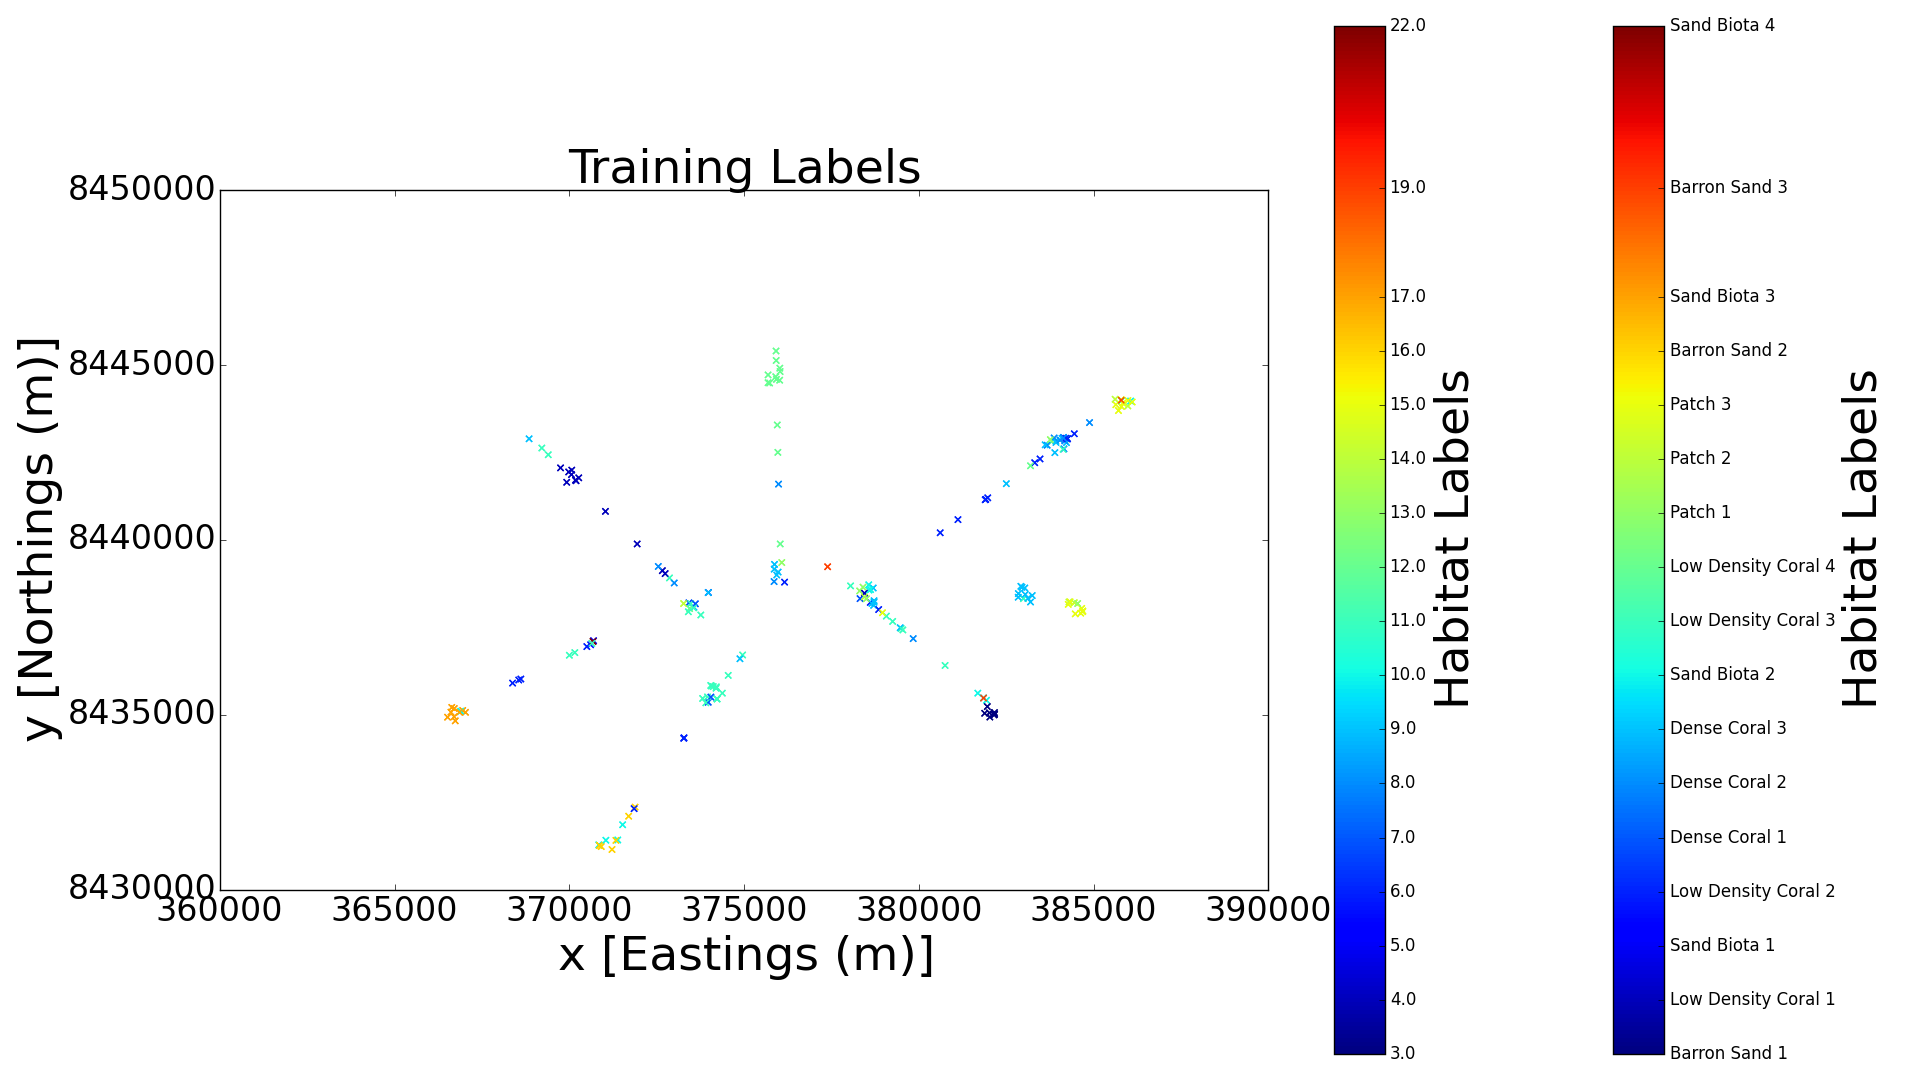
\includegraphics[width = 0.32\linewidth]{Figures/scott_reef_modeling/Figure1.png}
		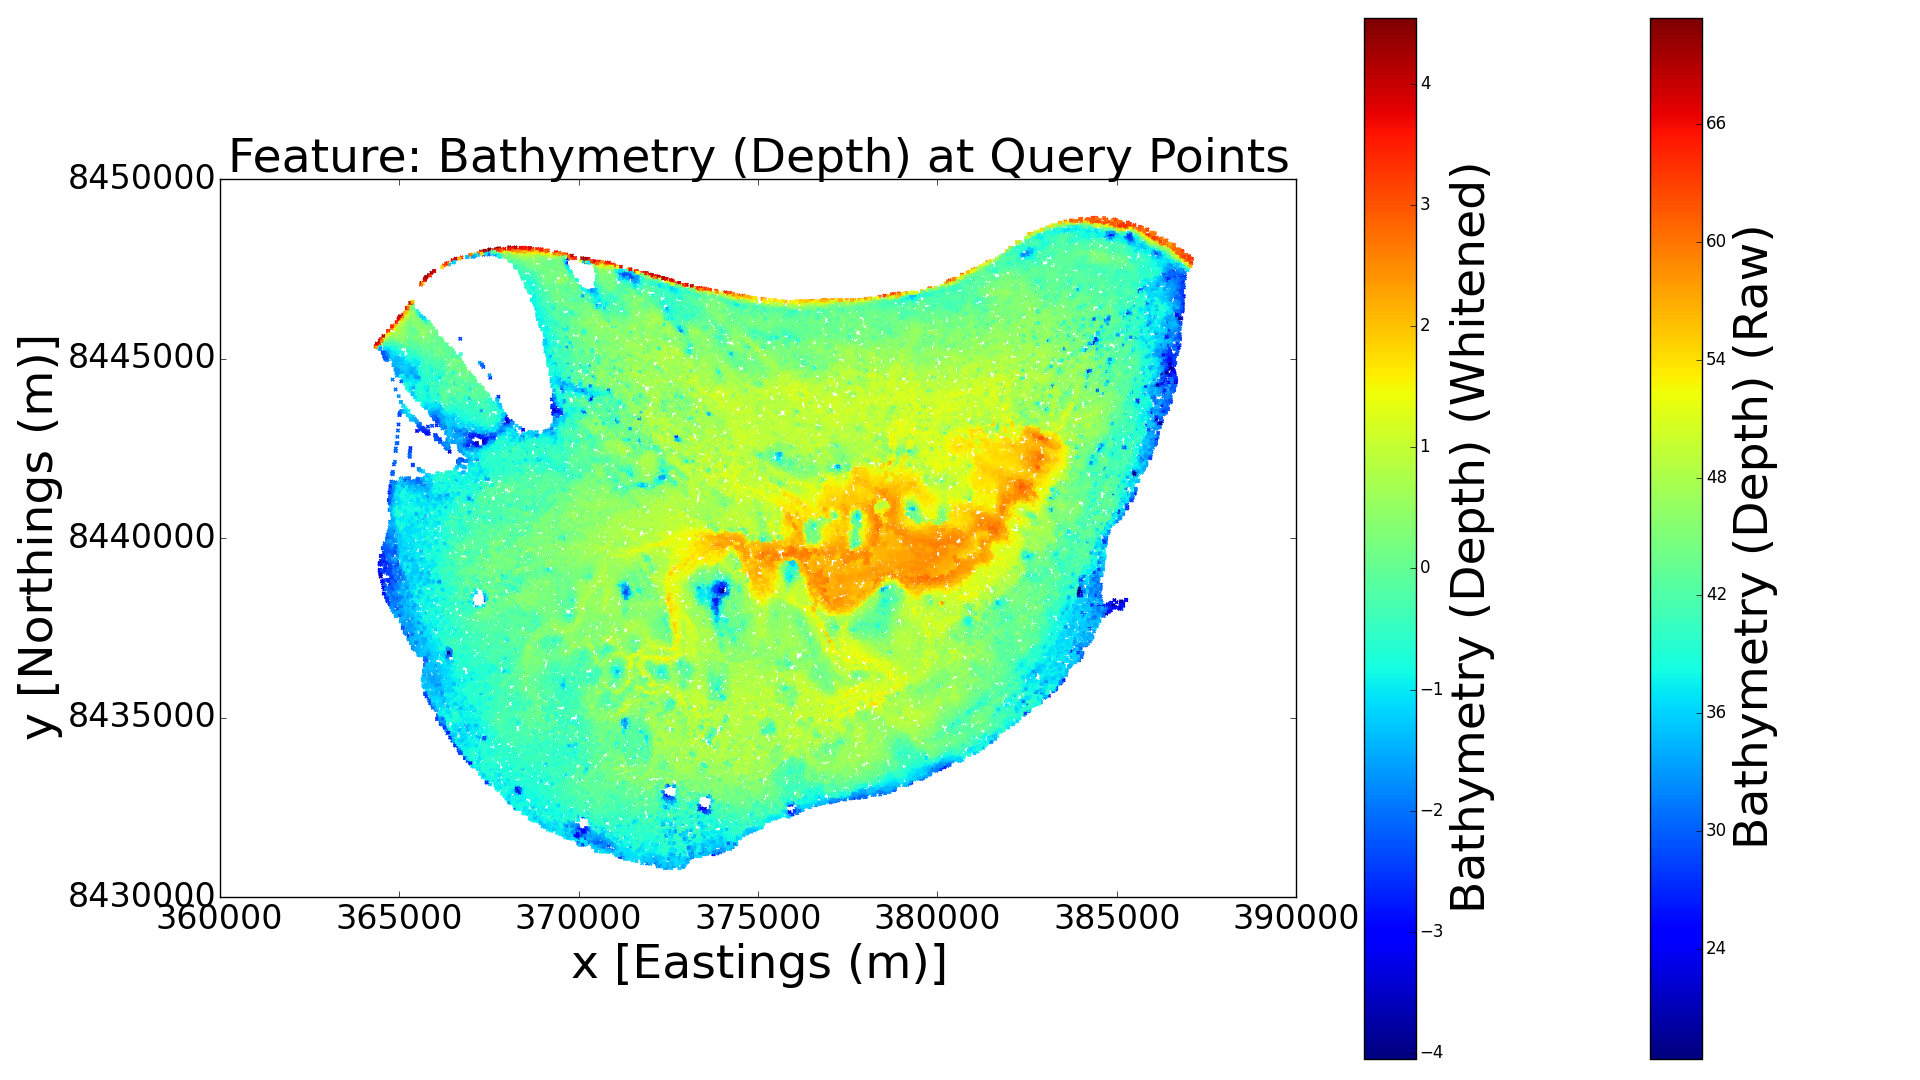
\includegraphics[width = 0.32\linewidth]{Figures/scott_reef_modeling/Figure2.png}
		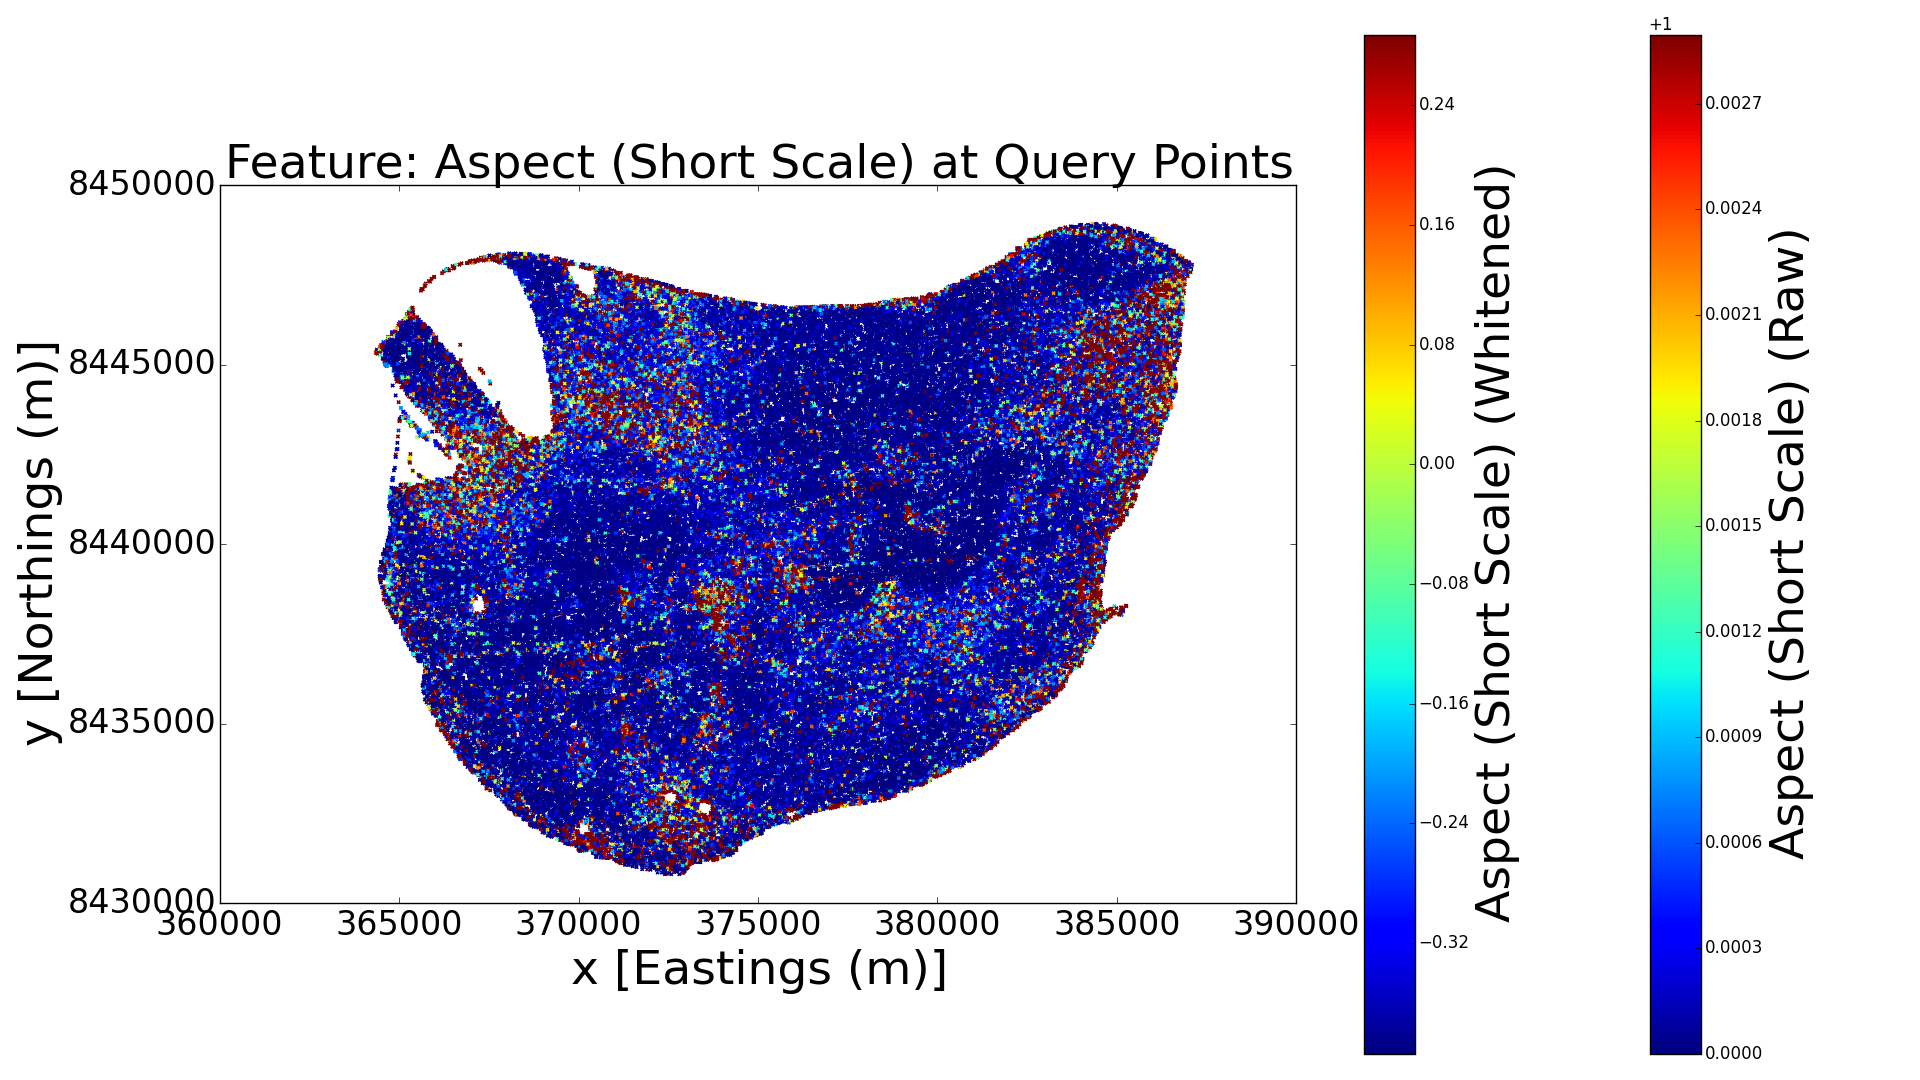
\includegraphics[width = 0.32\linewidth]{Figures/scott_reef_modeling/Figure3.png}
		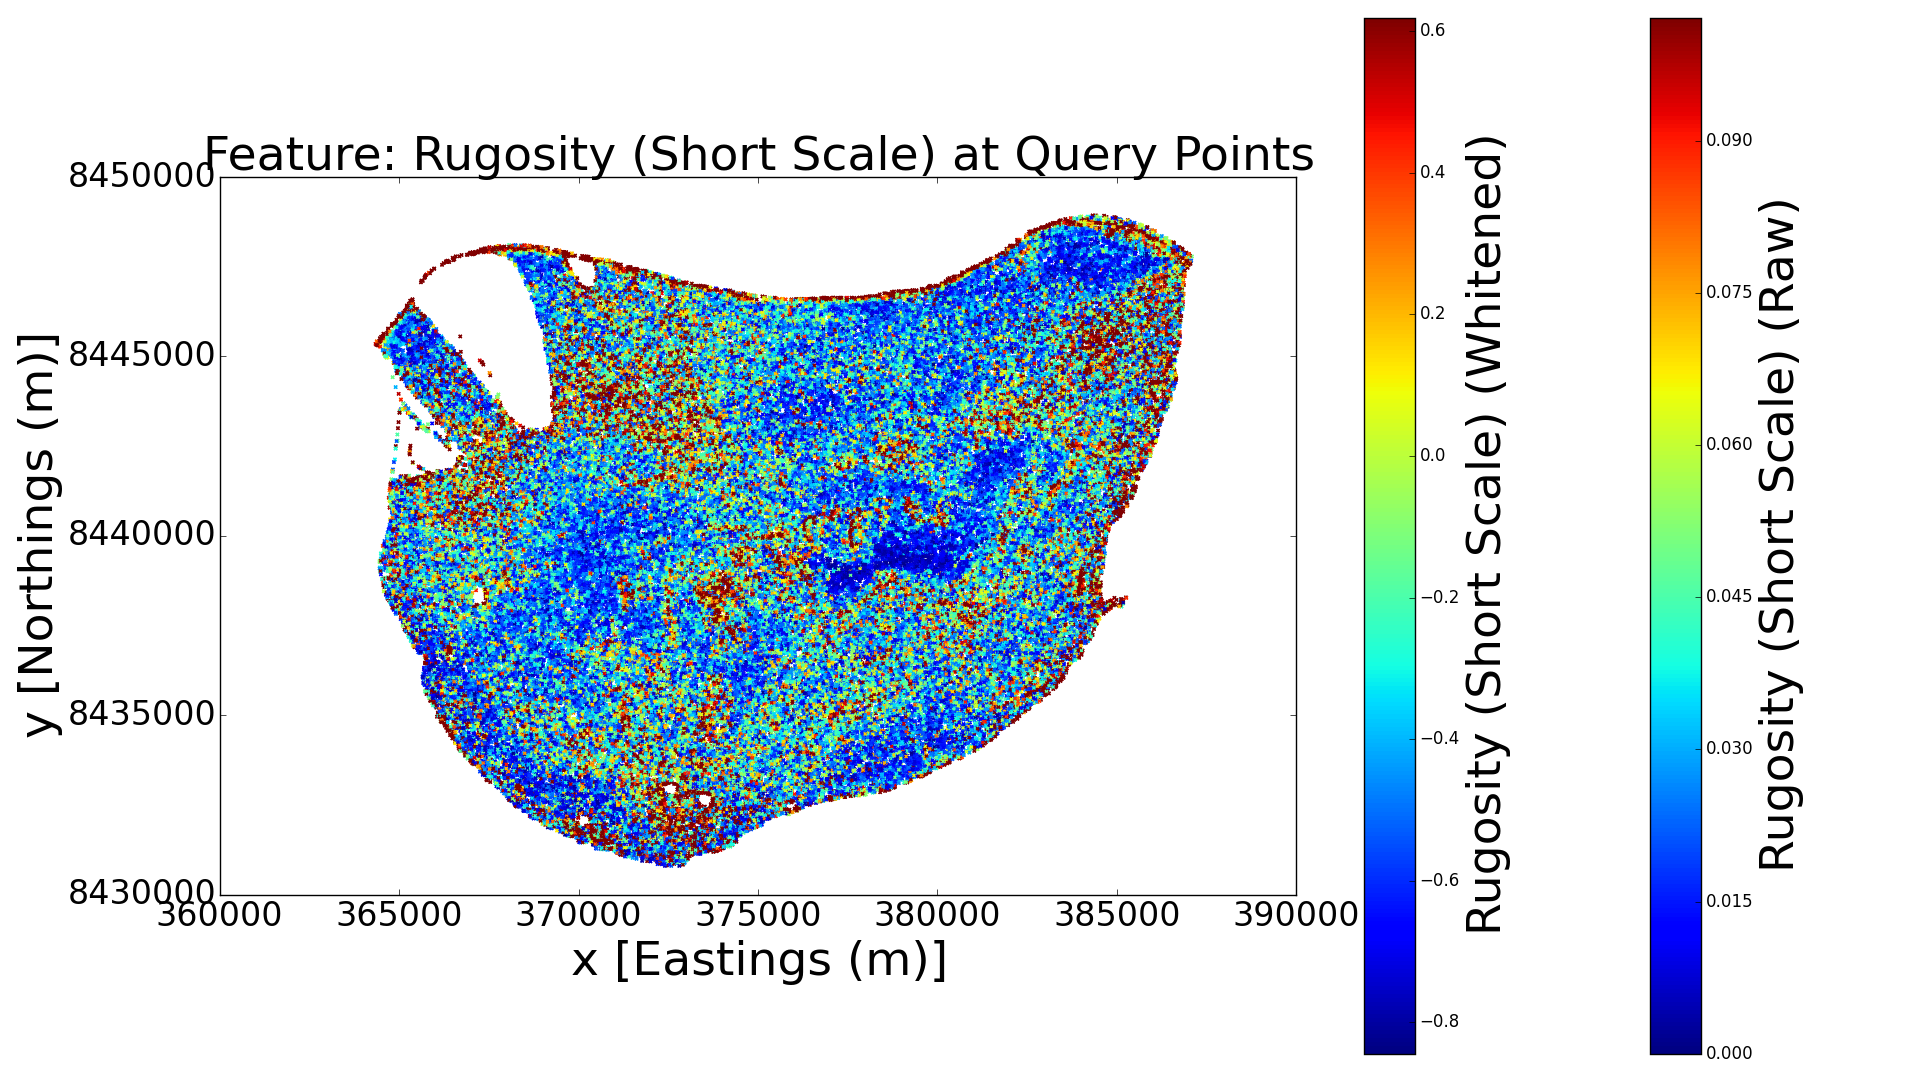
\includegraphics[width = 0.32\linewidth]{Figures/scott_reef_modeling/Figure4.png}
		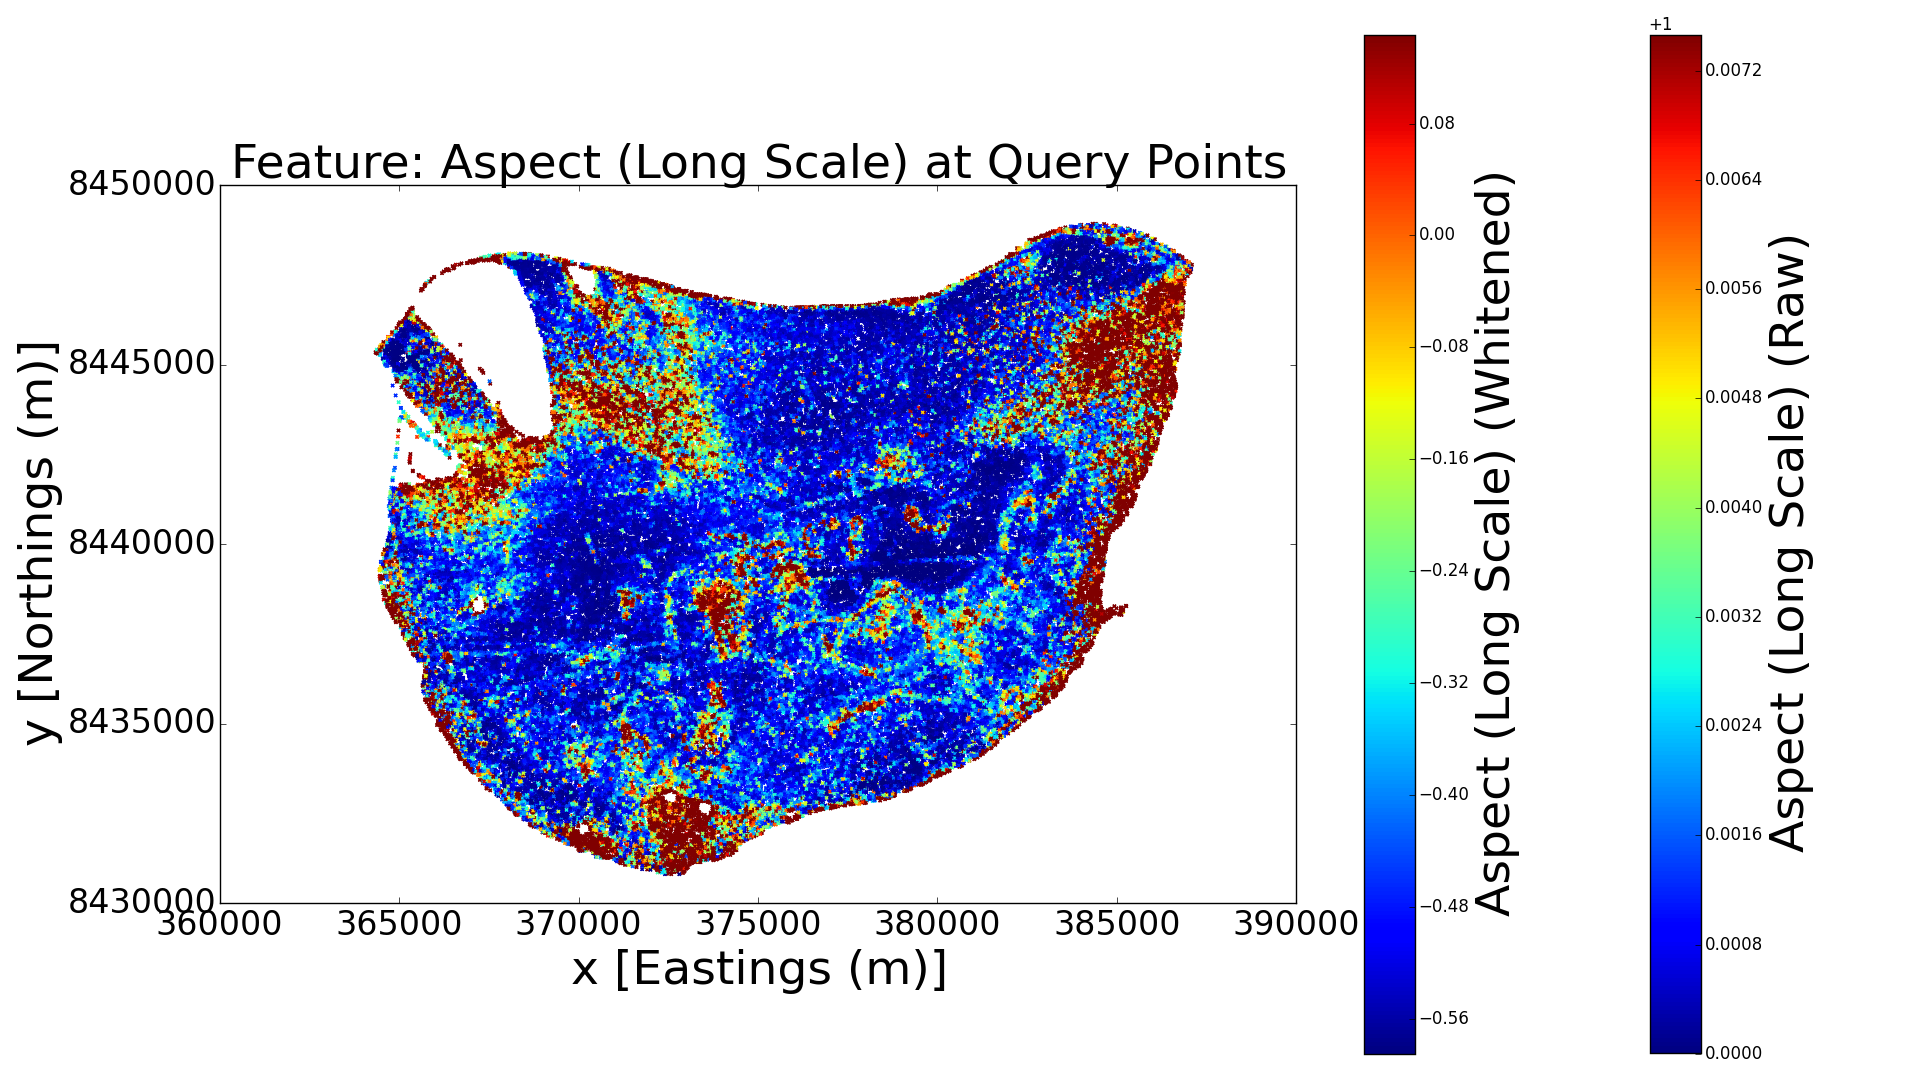
\includegraphics[width = 0.32\linewidth]{Figures/scott_reef_modeling/Figure5.png}
		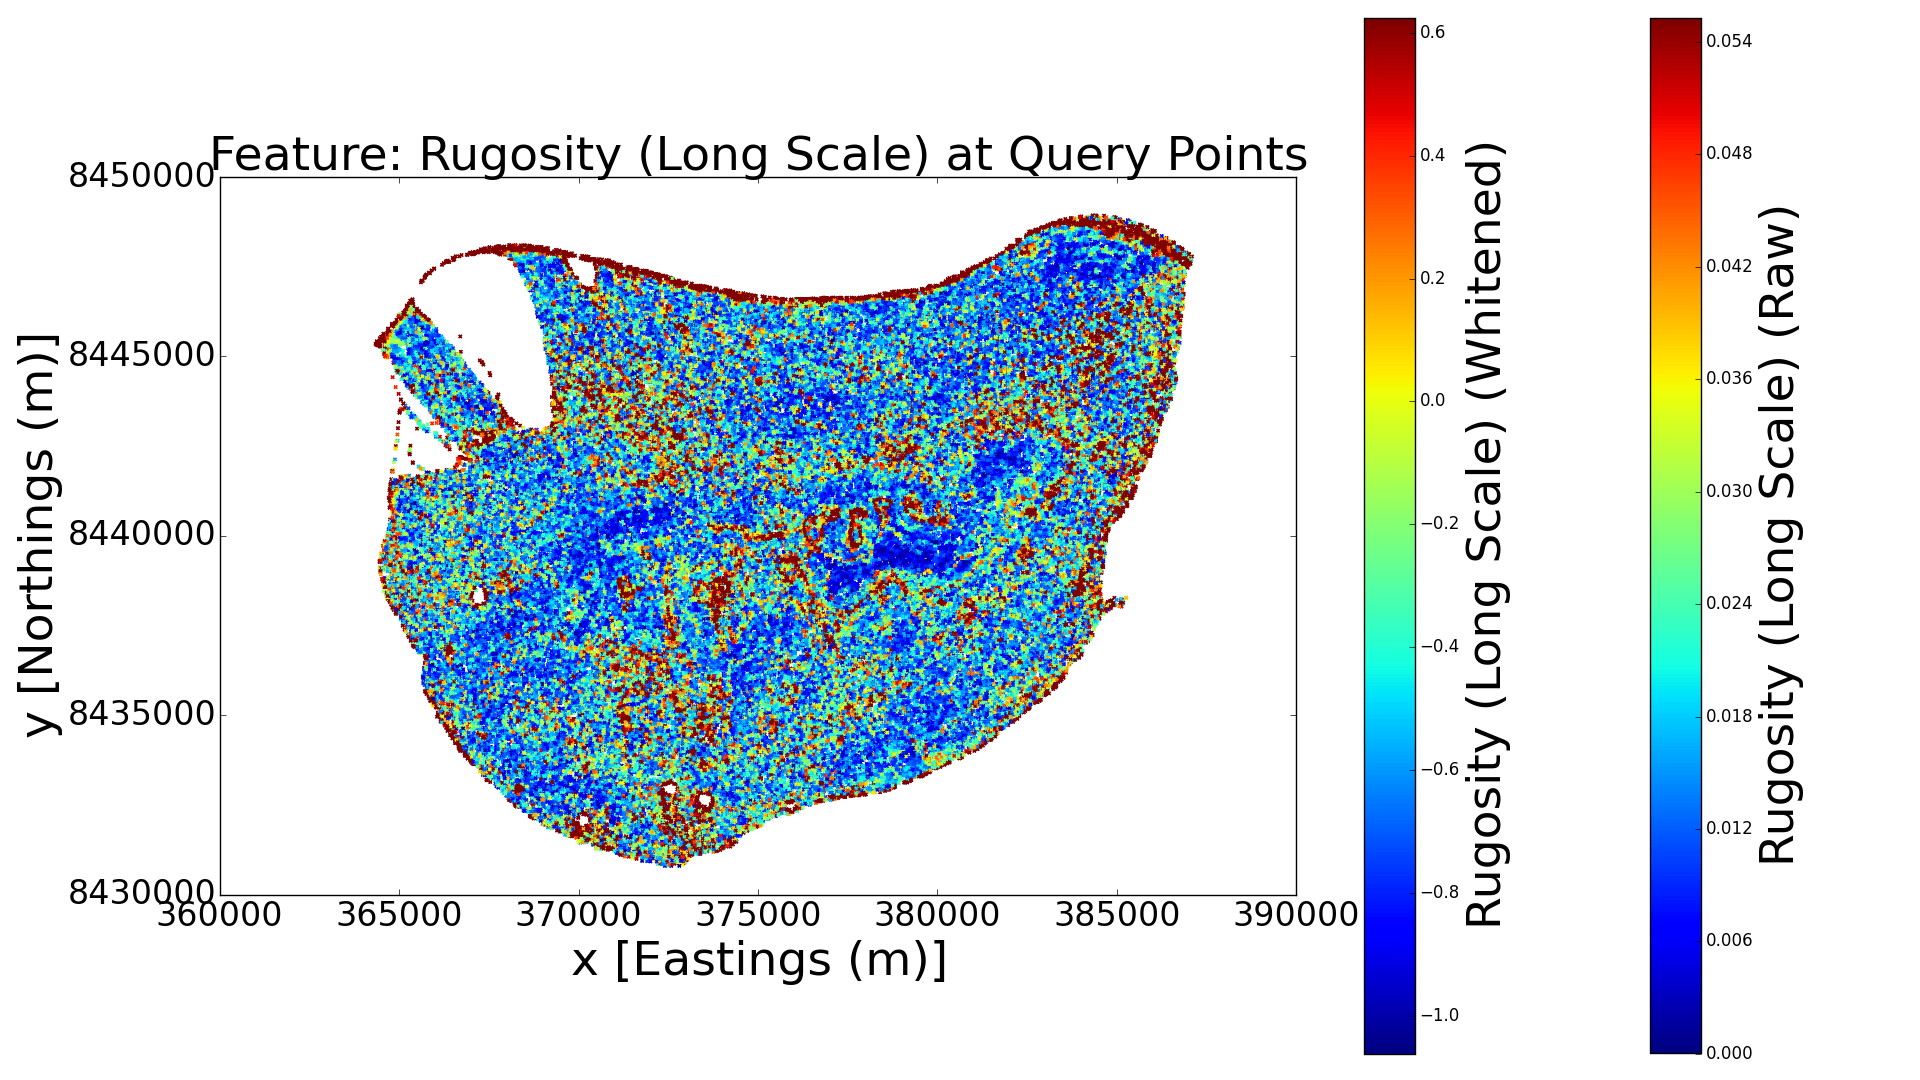
\includegraphics[width = 0.32\linewidth]{Figures/scott_reef_modeling/Figure6.png}
	\caption{Scott Reef Bathymetric Features}
	\label{Figure:Results:ScottReefBathymetricFeatures}
	\end{figure*}
	
	In this paper we will focus on applying the modeling and path planning techniques on the datasets collected from past missions at Scott Reefs, Western Australia \cite{ScottReefData}. While the dataset consists of a detailed map of the bathymetric features across the seafloor, the benthic habitats have only been observed through seven linear tracks extending from the middle to the edge of the reef (figure \ref{Figure:Results:ScottReefBathymetricFeatures}). The aim is to distinguish between the 17 different benthic zones and map the benthic habitats of the Scott reef region accurately in the shortest amount of travel time.
		
	\subsection{Model Structure and Features}
	
		Subplot 1 in figure \ref{Figure:Results:ScottReefBathymetricFeatures} shows the observed benthic habitats from past mission tracks, which serves as the training labels to our model. To reduce computational time, 200 training points were sampled from those tracks.
		
		Subplot 2 to 6 in figure \ref{Figure:Results:ScottReefBathymetricFeatures} shows the five bathymetric features for which the Gaussian process classifier will model upon - bathymetric depth, aspect (short and long scale), rugosity (short and long scale). The images are built from 10000 query points randomly sampled from the dataset.
		
		To measure the relative performance between modeling and path planning techniques, a synthetic ground truth is generated separately (figure \ref{Figure:Results:ScottReefSyntheticTruth}). Note that this ground truth was generated using a separate sample of the training tracks and does not necessary represent the true benthic regions at Scott reef.
	



					
	\subsection{Gaussian Processes Classifiers}
	
		\begin{figure}[!htbp]
		\centering
			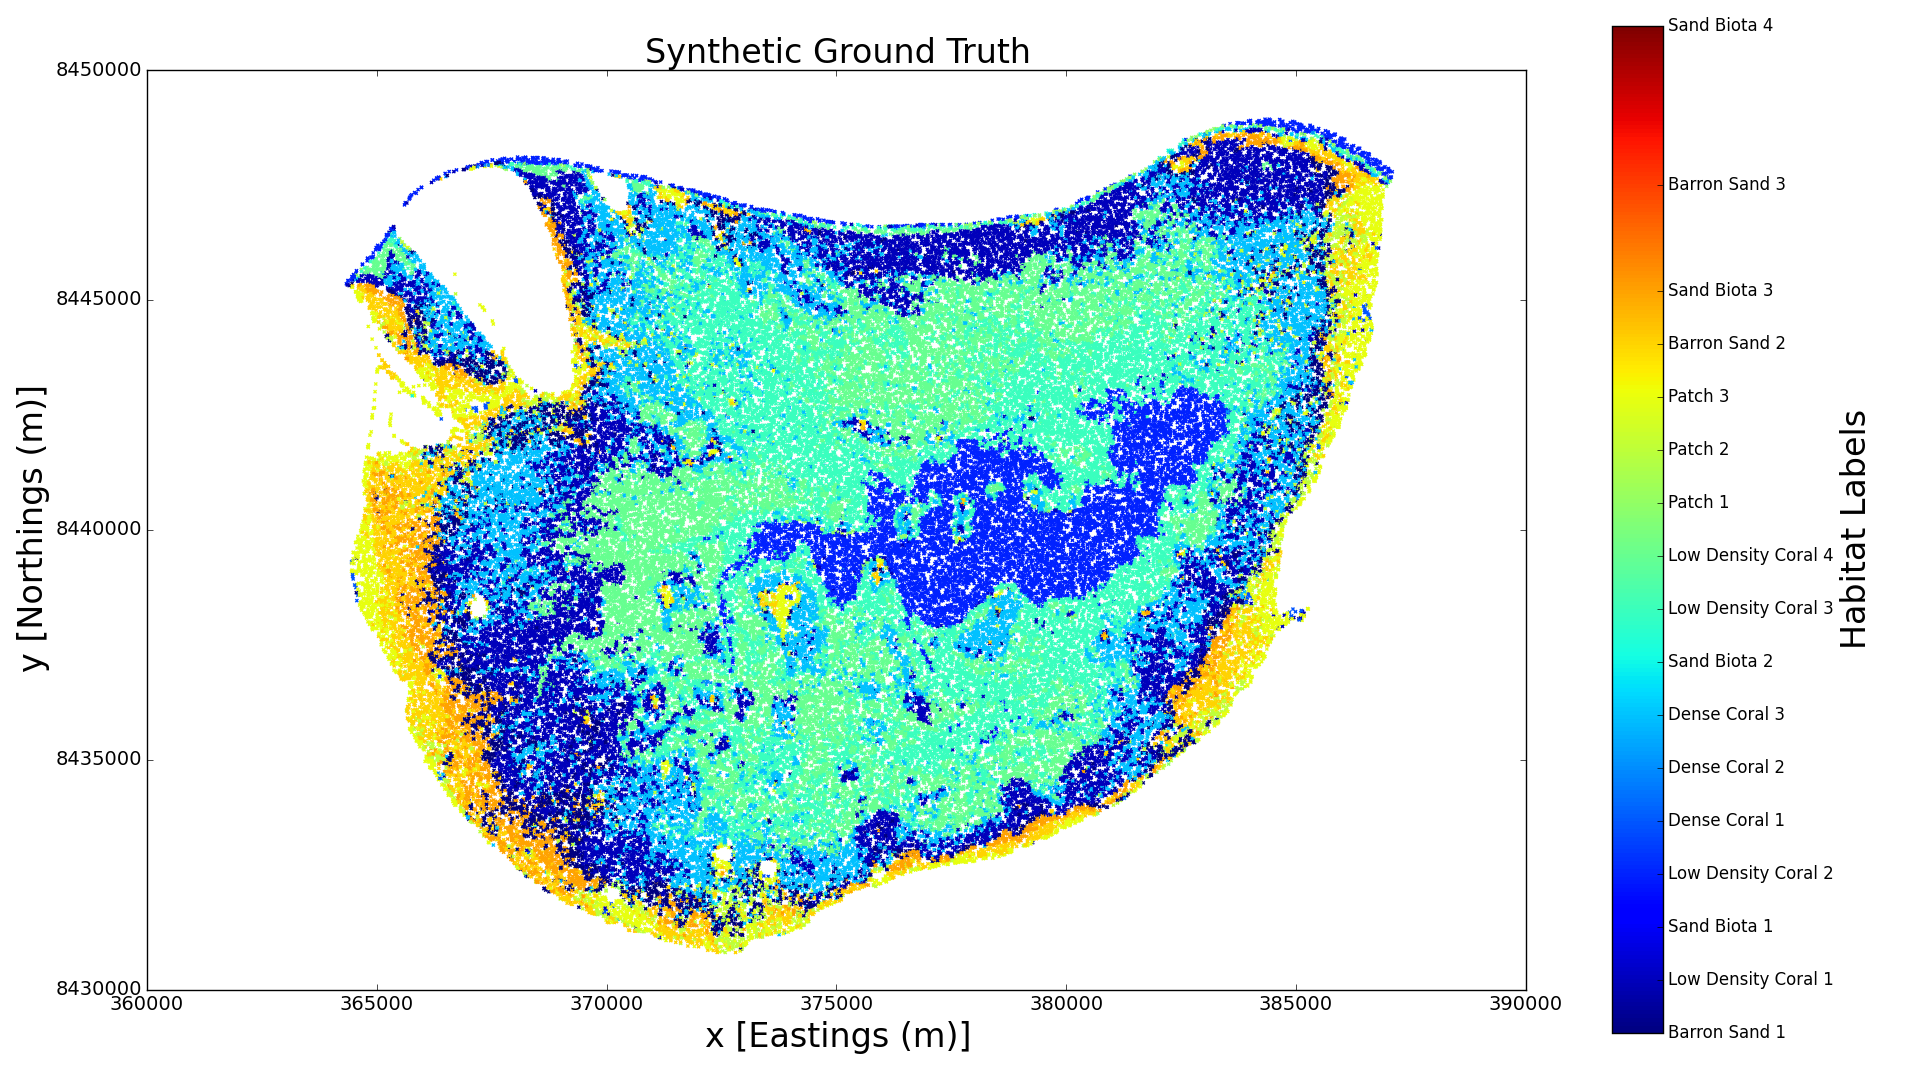
\includegraphics[width = \linewidth]{Figures/scott_reef_modeling/Figure7.png}
		\caption{Scott Reef: Synthetic Ground Truth}
		\label{Figure:Results:ScottReefSyntheticTruth}
		\end{figure}

		\begin{figure}[!htbp]
		\centering
			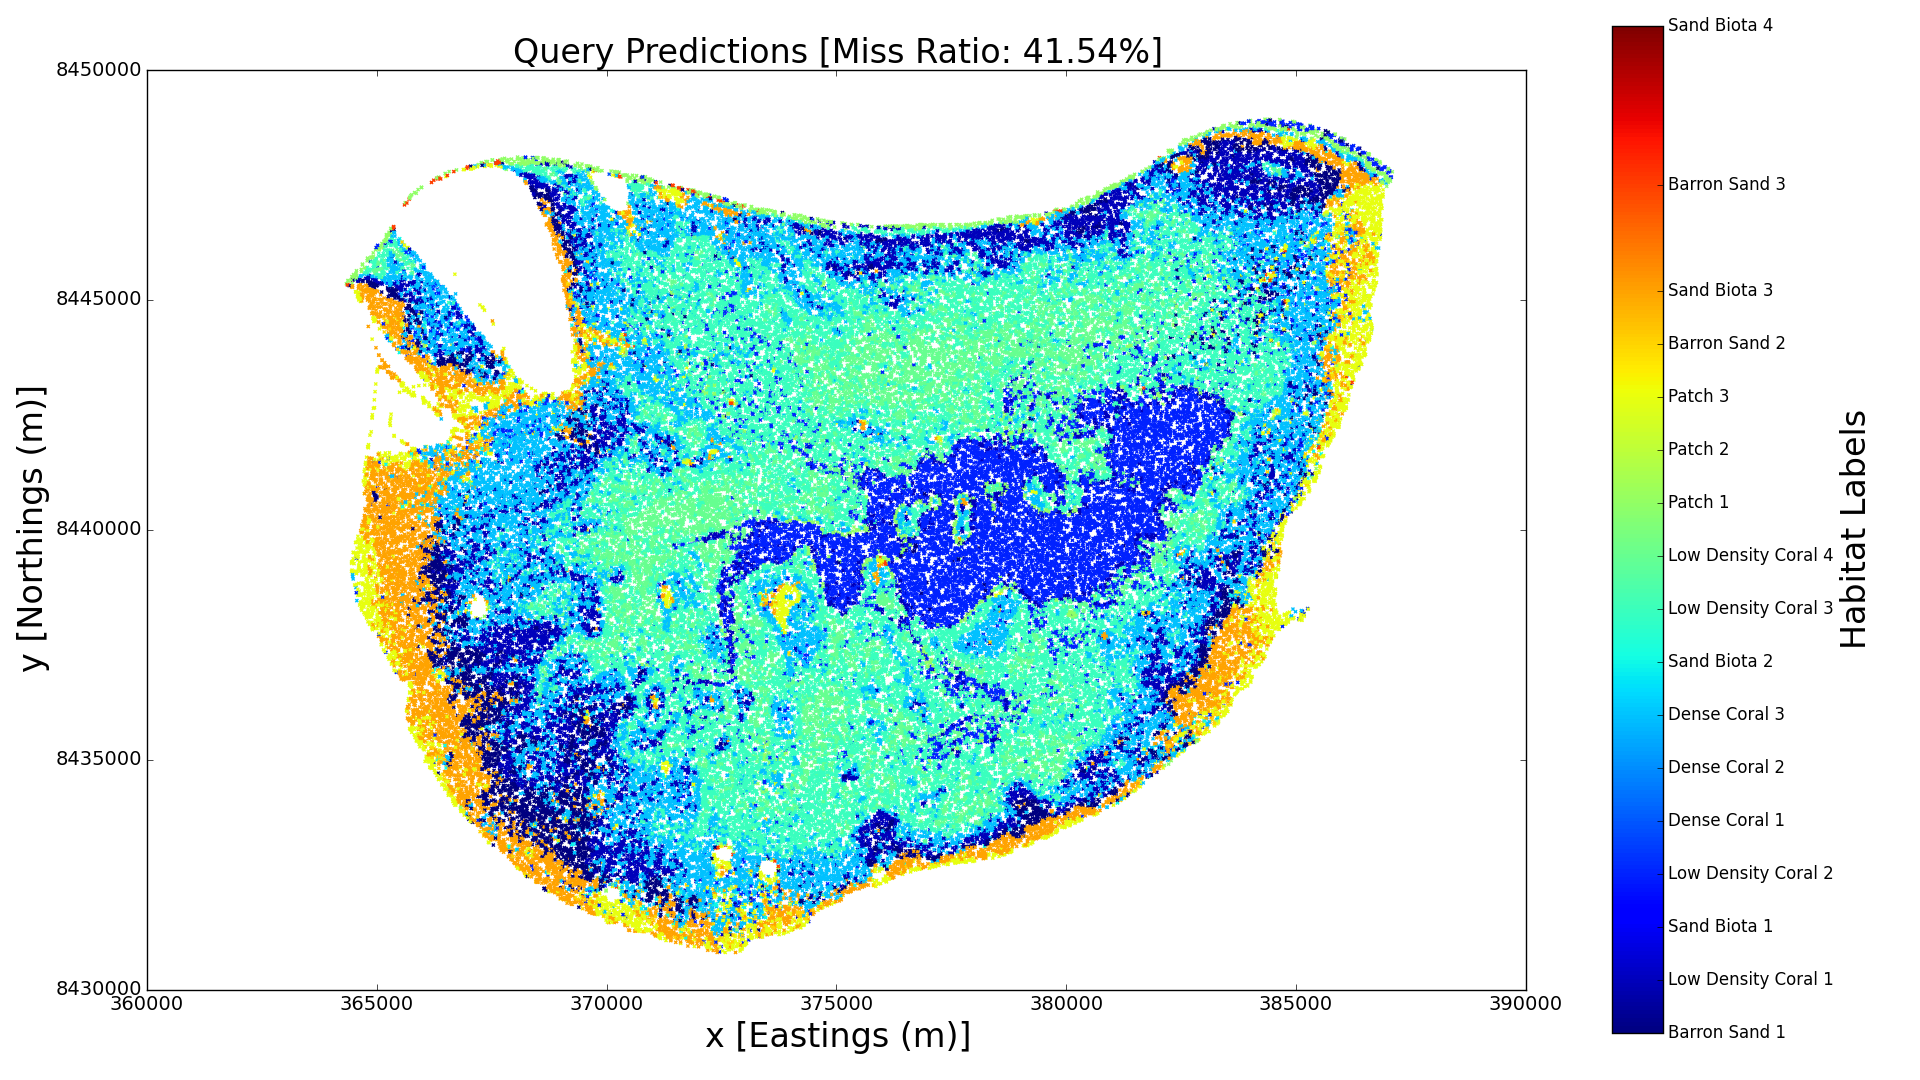
\includegraphics[width = \linewidth]{Figures/scott_reef_modeling/Figure8.png}
		\caption{Scott Reef: Initial Prediction with 200 Training Points}
		\label{Figure:Results:ScottReefPredictions}
		\end{figure}
	
		\begin{figure}[!htbp]
		\centering
			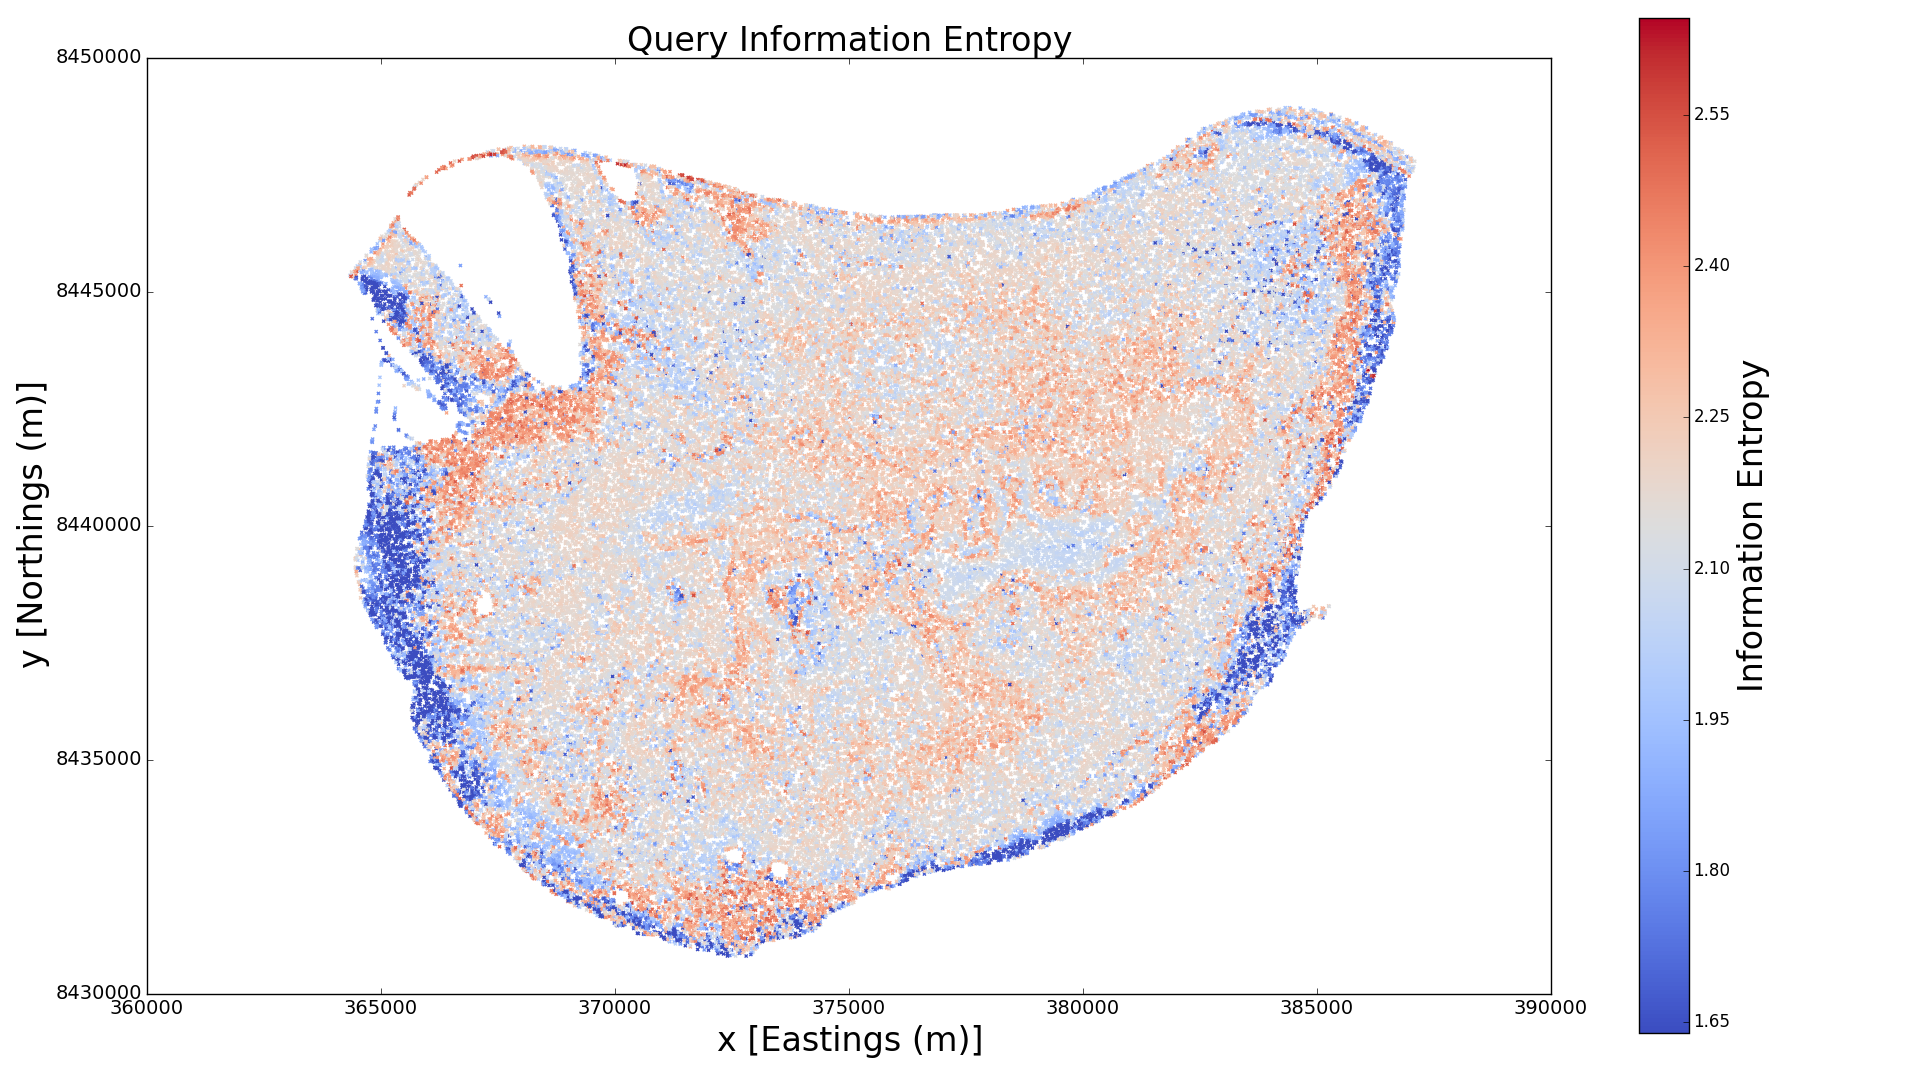
\includegraphics[width = \linewidth]{Figures/scott_reef_modeling/Figure9.png}
		\caption{Scott Reef: Prediction Information Entropy}
		\label{Figure:Results:ScottReefPredictionInformationEntropy}
		\end{figure}
		
		\begin{figure}[!htbp]
		\centering
			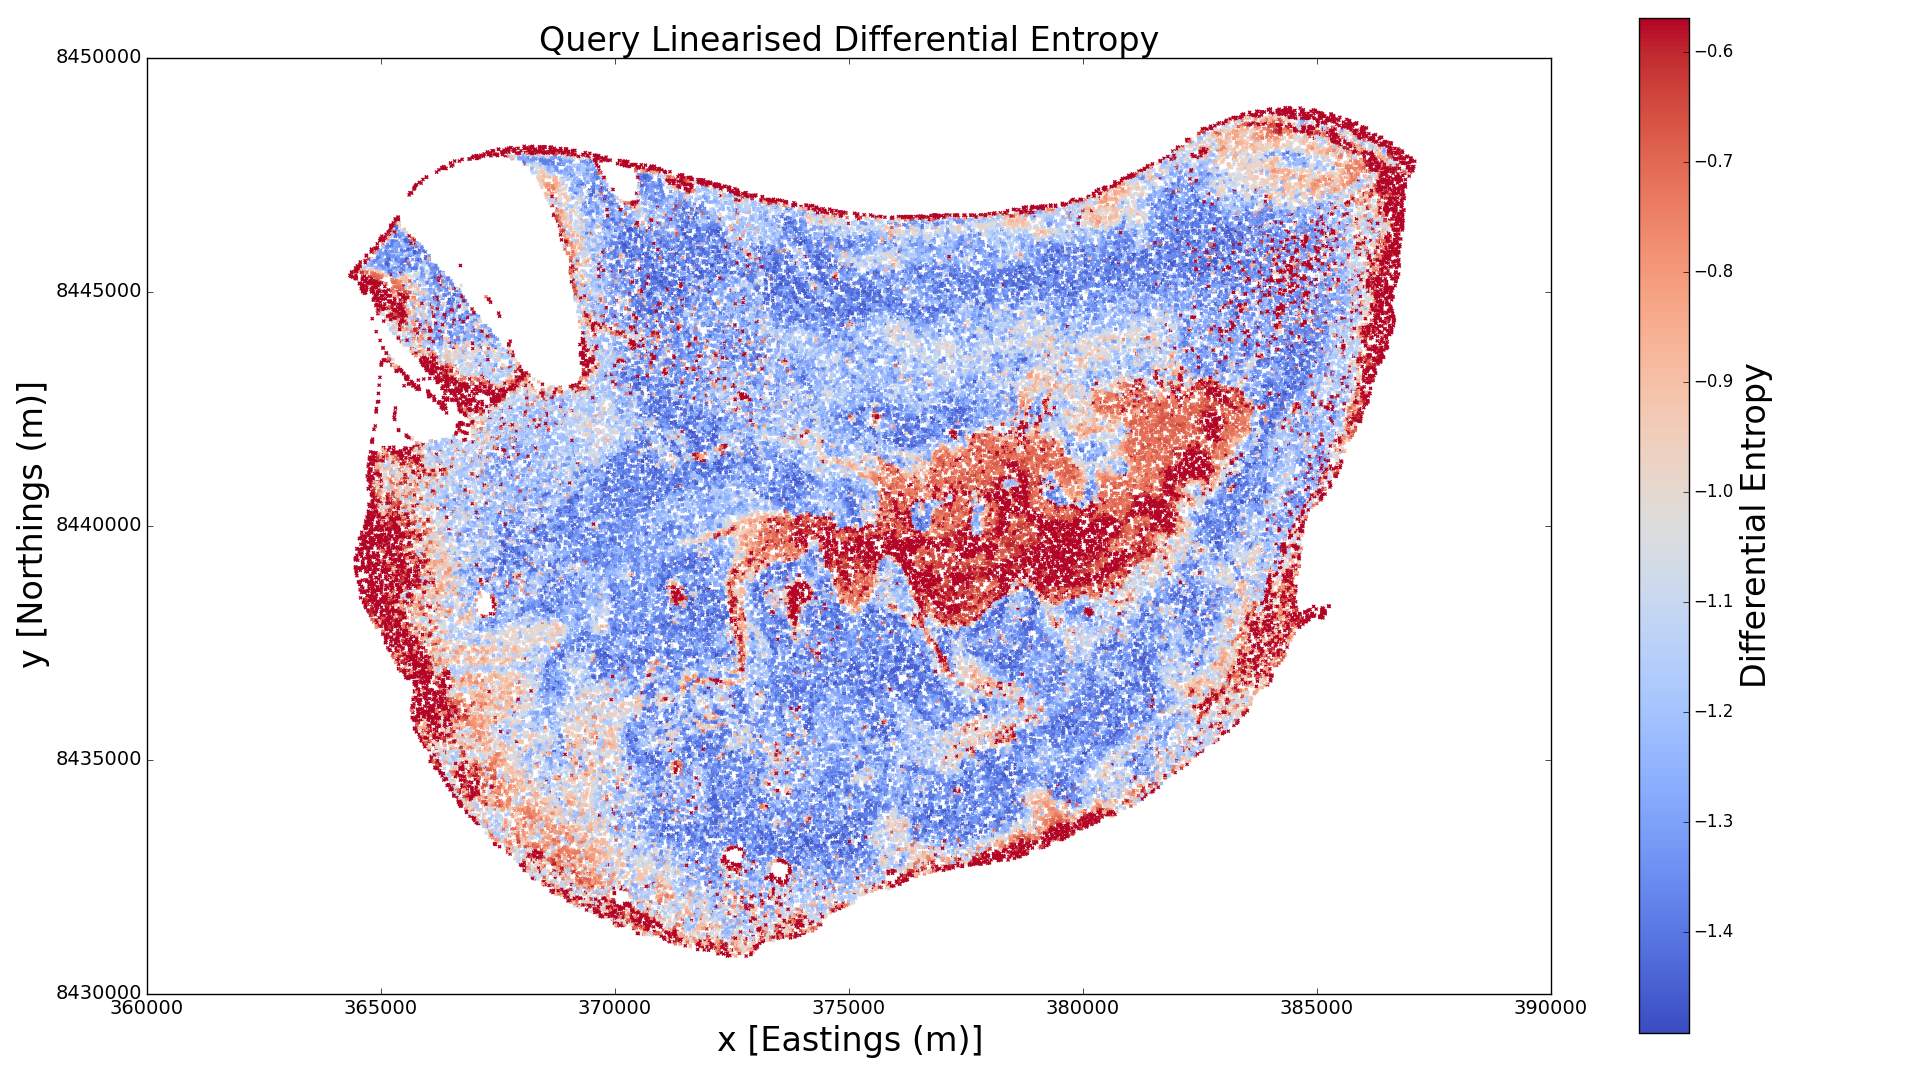
\includegraphics[width = \linewidth]{Figures/scott_reef_modeling/Figure11.png}
		\caption{Scott Reef: Linearised Differential Entropy}
		\label{Figure:Results:ScottReefLinearisedDifferentialEntropy}
		\end{figure}
					
		{\color{BurntOrange} This is a random paragraph of stuff. I talk about things. This is just a filler paragraph. Today is sunny. Rainbows are colorful. Blah blah blah.}
		
		{\color{BurntOrange} This is a random paragraph of stuff. I talk about things. This is just a filler paragraph. Today is sunny. Rainbows are colorful. Blah blah blah.}
		
		{\color{BurntOrange} This is a random paragraph of stuff. I talk about things. This is just a filler paragraph. Today is sunny. Rainbows are colorful. Blah blah blah.}
		
		{\color{BurntOrange} This is a random paragraph of stuff. I talk about things. This is just a filler paragraph. Today is sunny. Rainbows are colorful. Blah blah blah.}
		
		{\color{BurntOrange} This is a random paragraph of stuff. I talk about things. This is just a filler paragraph. Today is sunny. Rainbows are colorful. Blah blah blah.}
		
		{\color{BurntOrange} This is a random paragraph of stuff. I talk about things. This is just a filler paragraph. Today is sunny. Rainbows are colorful. Blah blah blah.}
		
		{\color{BurntOrange} This is a random paragraph of stuff. I talk about things. This is just a filler paragraph. Today is sunny. Rainbows are colorful. Blah blah blah.}
		
		{\color{BurntOrange} This is a random paragraph of stuff. I talk about things. This is just a filler paragraph. Today is sunny. Rainbows are colorful. Blah blah blah.}
		
		{\color{BurntOrange} This is a random paragraph of stuff. I talk about things. This is just a filler paragraph. Today is sunny. Rainbows are colorful. Blah blah blah.}
		
		{\color{BurntOrange} This is a random paragraph of stuff. I talk about things. This is just a filler paragraph. Today is sunny. Rainbows are colorful. Blah blah blah.}
		
		{\color{BurntOrange} This is a random paragraph of stuff. I talk about things. This is just a filler paragraph. Today is sunny. Rainbows are colorful. Blah blah blah.}
		
		{\color{BurntOrange} This is a random paragraph of stuff. I talk about things. This is just a filler paragraph. Today is sunny. Rainbows are colorful. Blah blah blah.}
		
		{\color{BurntOrange} This is a random paragraph of stuff. I talk about things. This is just a filler paragraph. Today is sunny. Rainbows are colorful. Blah blah blah.}
		
		{\color{BurntOrange} This is a random paragraph of stuff. I talk about things. This is just a filler paragraph. Today is sunny. Rainbows are colorful. Blah blah blah.}
		
		{\color{BurntOrange} This is a random paragraph of stuff. I talk about things. This is just a filler paragraph. Today is sunny. Rainbows are colorful. Blah blah blah.}
		
		
		\begin{figure}[!htbp]
			\centering
				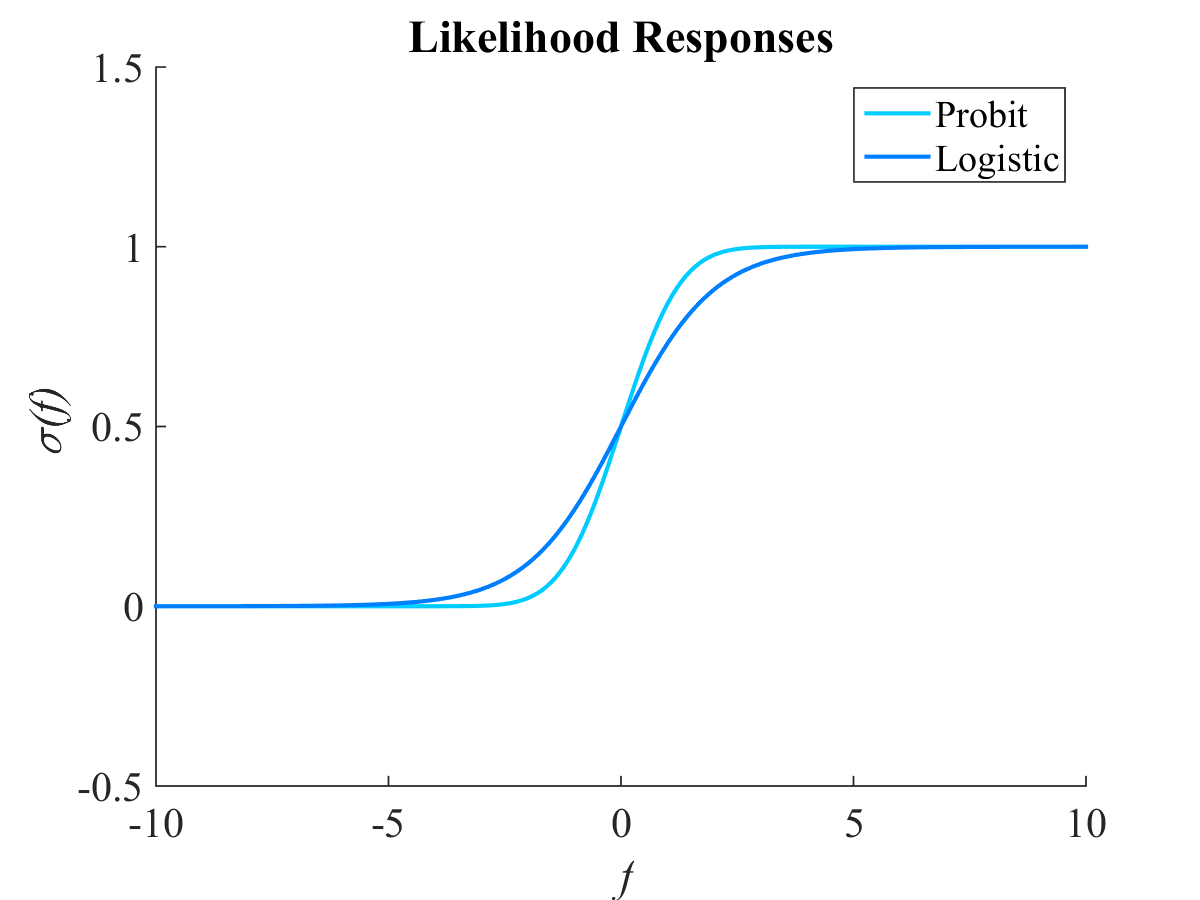
\includegraphics[width = \linewidth]{Figures/responses.png}
			\caption{Likelihood Responses}
			\label{Figure:LikelihoodResponses}
		\end{figure}
	
		{\color{BurntOrange} This is a random paragraph of stuff. I talk about things. This is just a filler paragraph. Today is sunny. Rainbows are colorful. Blah blah blah.}
		
		{\color{BurntOrange} This is a random paragraph of stuff. I talk about things. This is just a filler paragraph. Today is sunny. Rainbows are colorful. Blah blah blah.}
		
		{\color{BurntOrange} This is a random paragraph of stuff. I talk about things. This is just a filler paragraph. Today is sunny. Rainbows are colorful. Blah blah blah.}
		
		{\color{BurntOrange} This is a random paragraph of stuff. I talk about things. This is just a filler paragraph. Today is sunny. Rainbows are colorful. Blah blah blah.}
		
		{\color{BurntOrange} This is a random paragraph of stuff. I talk about things. This is just a filler paragraph. Today is sunny. Rainbows are colorful. Blah blah blah.}
		
\section{Linearised Differential Entropy of Gaussian Process Classifiers}
\label{Section:LinearisedEntropy}

	In this section we introduce the linearised differential entropy of Gaussian process classifiers. This method attempts to address the need for a measure of mutual entropy that is more computationally viable compared to Monte Carlo methods. We motivate the properties that such a measure much have, and proceed to define and derive such a measure. Finally, we visualise its advantage through simple tests cases in both the binary and multiclass classification setting.
	
	\subsection{Binary Classification}

		For binary classification, linearisation is performed on the likelihood response function.
	
		Suppose we have trained our Gaussian process classifier using Laplace approximation with respect to a training set $\mathcal{D} = \{X, \vec{y}\} = \{[ \vec{x}_{1}, \vec{x}_{2}, \dots, \vec{x}_{n}]^{T}, [y_{1}, y_{2}, \dots, y_{n}]\}$ with $n$ training points. We know that the latent function $f(\vec{x})$ is distributed as a GP with a particular predictive mean $m(\vec{x})$ and covariance $k(\vec{x}, \vec{x}')$ once conditioned on the training data \eqref{Section:LinearisedEntropy:Equation:PredictiveGP}. From here on we omit explicitly notating the training set that was conditioned upon.
		
		\begin{equation}
			f(\vec{x}) \sim \mathcal{GP}(m(\vec{x}), k(\vec{x}, \vec{x}'))
		\label{Section:LinearisedEntropy:Equation:PredictiveGP}
		\end{equation}
		
		Let $X^{\star} = [ \vec{x}^{\star}_{1}, \vec{x}^{\star}_{2}, \dots, \vec{x}^{\star}_{n^{\star}}]^{T}$ denote the collection of $n^{\star}$ query points for which inference is to be performed. Denote $\vec{f}^{\star}$ the vector of latent function values $f^{\star}_{i} = f(\vec{x}^{\star}_{i})$ at each query point. We have by definition of a GP that $\vec{f}^{\star}$ is multivariate Gaussian distributed with a corresponding means $\mu^{\star}_{i} = m(\vec{x}^{\star}_{i})$ and covariances $\Sigma^{\star}_{ij} = k(\vec{x}^{\star}_{i}, \vec{x}^{\star}_{j})$ \eqref{Section:LinearisedEntropy:Equation:PredictiveGaussianDistribution}.
		
		\begin{equation}
			\vec{f}^{\star} = [f^{\star}_{1}, f^{\star}_{2}, \dots, f^{\star}_{n^{\star}}]^{T} \sim \mathcal{N}(\vec{\mu}^{\star}, \Sigma^{\star})
		\label{Section:LinearisedEntropy:Equation:PredictiveGaussianDistribution}
		\end{equation}
			
		The binary prediction probability $\vec{\pi^{\star}}$ at the query points is obtained through passing the queried latent function random vector $\vec{f}^{\star}$ through a response function in a component wise fashion \eqref{Section:LinearisedEntropy:Equation:Response}.
		
		\begin{equation}
			\vec{\pi}^{\star} = \vec{\sigma}(f^{\star})\mathrm{ \qquad i.e. \;\;}\pi^{\star}_{i} = \sigma(f^{\star}_{i}) \qquad \forall i \in \{1, 2, \dots, n^{\star}\}
		\label{Section:LinearisedEntropy:Equation:Response}
		\end{equation}
		
		As a straightforward transformation of the latent vector, the predictive probability vector $\vec{\pi^{\star}}$ is thus a random vector itself. The usual procedure is then to treat the expected predition probabilities $\mathbb{E}(\vec{\pi^{\star}})$ as the posterior class probabilities for further inference. However, this discards any information regarding the joint behaviour at the query points. As a result, a measure of mutual information shared amongst the query points cannot be obtained.
		
		One straightforward approach to address this problem is to perform Monte Carlo estimation of the posterior joint distribution for class predictions via jointly sampling latent vectors from the GP, assigning class label 1 for positive latent values and -1 otherwise, and compute the Shannon entropy \cite{ShannonEntropy} from the estimated joint distribution. Aside from the relatively long computational time required for sampling enough draws for accurate joint distribution estimation, the Monte Carlo approach also has the tendency to overestimate variances at locations with low densities of training observations.
				
		Instead, we propose using the joint distribution of the predictive probabilities $\vec{\pi^{\star}}$ itself as a basis of constructing a measure of mutual information. Unlike traditional approaches where inference depends only on the expectance $\mathbb{E}(\vec{\pi^{\star}})$ such that structural information from the latent GP is compromised, we utilise also the covariance $\mathbb{V}(\vec{\pi^{\star}})$, which withholds information regarding both the latent GP and the response likelihood.
	
		\begin{figure}[!htbp]
			\centering
				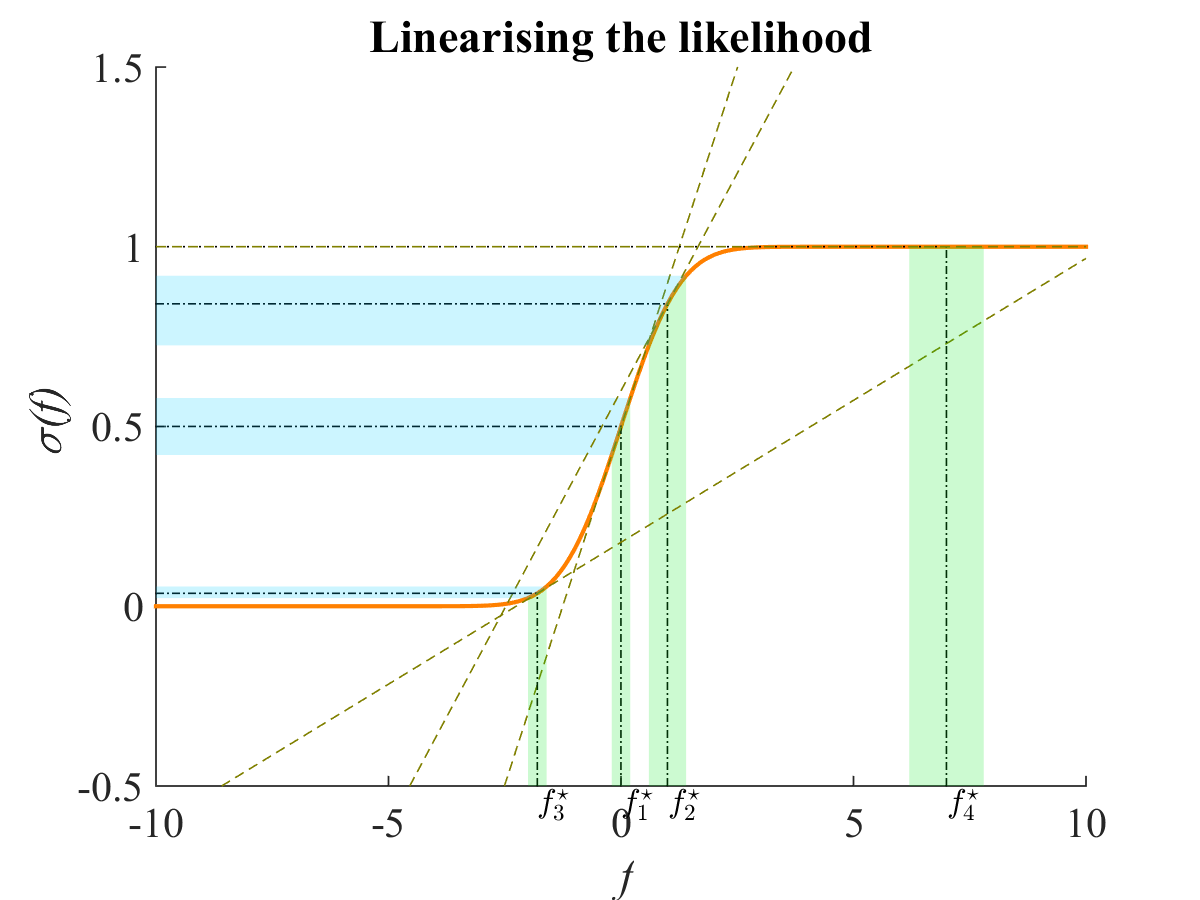
\includegraphics[width = \linewidth]{Figures/linearisation.png}
			\caption{Linearisation accuracy for a probit response: Green shade represents the latent variance while blue shade represents the predictive variance. Gold lines show local linearisation about latent expectance.}
			\label{Figure:Linearisation}
		\end{figure}
			
		As the predictive probabilities are nonlinear transformations (Figure \ref{Figure:LikelihoodResponses}) of the Gaussian distributed latent vector, they are no longer Gaussian distributed. Hence, we propose linearising the response function about the latent expectance $\bar{f}^{\star}_{i} := \mathbb{E}(f^{\star}_{i})$. Figure \ref{Figure:Linearisation} illustrates the linearisation accuracy for a probit response. Observe that points with latent expectance far away from zero translate to near zero predictive variance even under high latent variance. Linearisation is thus very accurate for those points. For points with latent expectances near zero, we require the latent variances to be sufficiently small for linearisation to be accurate.

		\begin{figure*}[tb]
		\centering
			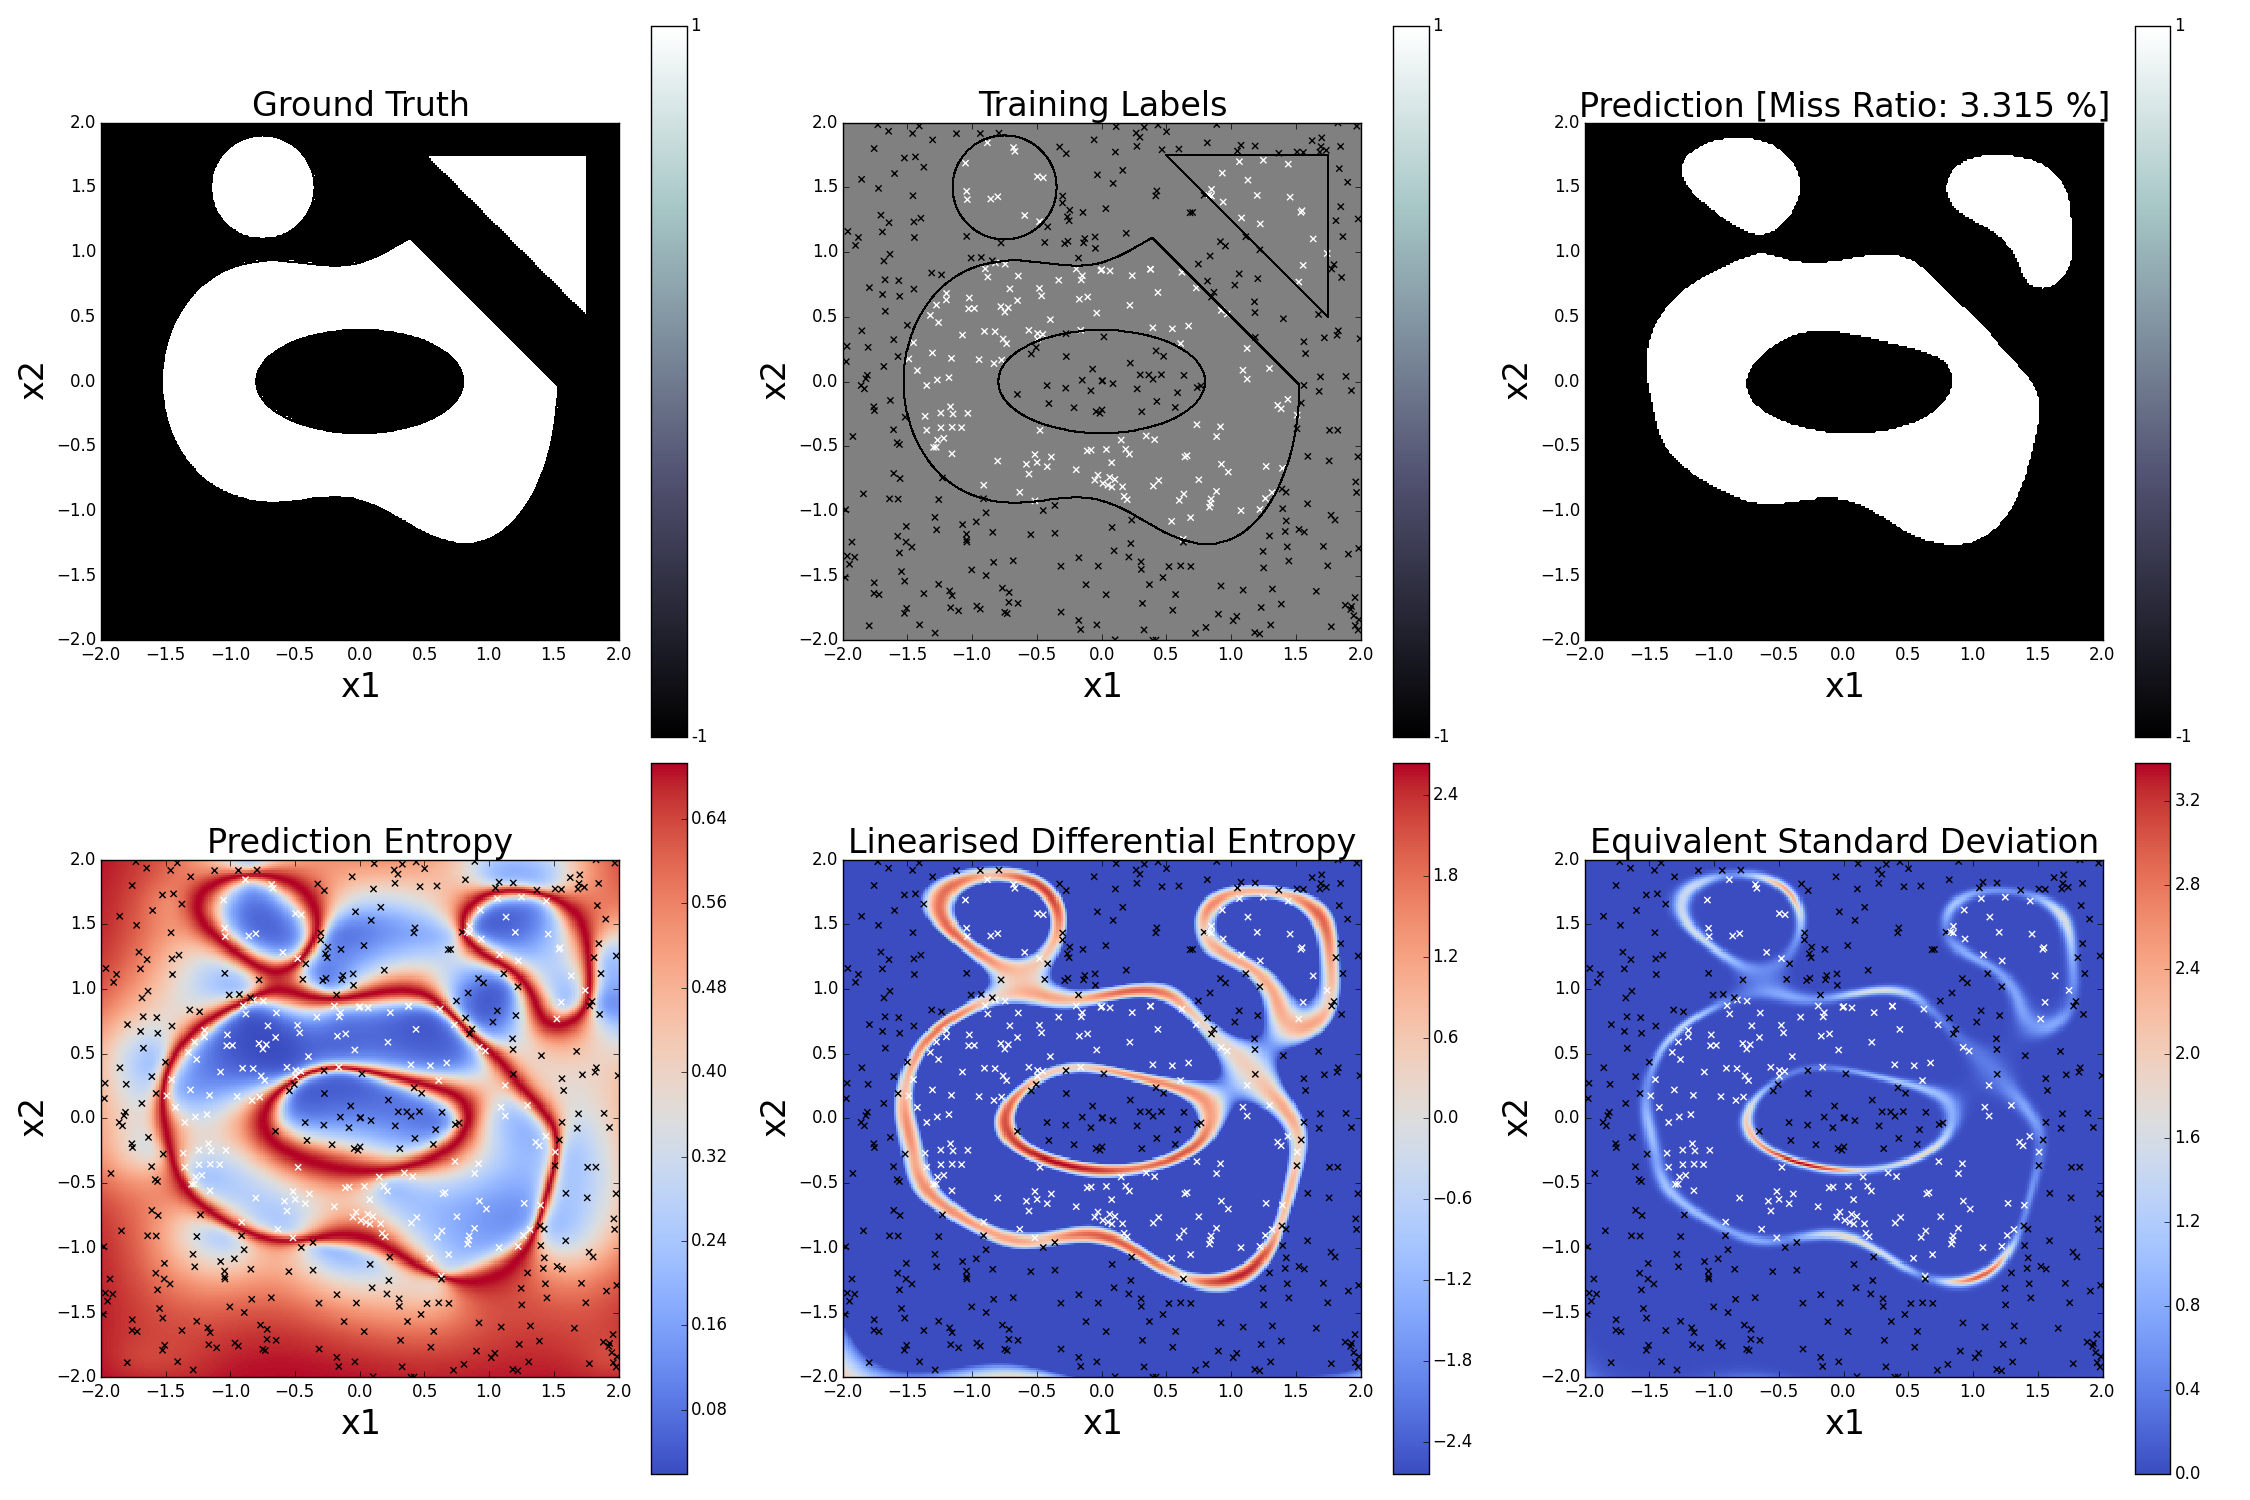
\includegraphics[width = \linewidth]{Figures/binary_linearised_entropy/Figure1.png}
		\caption{Example: Linearised Differential Entropy for a Binary Classifier}
		\label{Figure:Results:BinaryLinearisedEntropy}
		\end{figure*}
		
		\subsubsection{Derivation}
		
			We proceed to derive the linearisation which also serves to construct the definition of linearised differential entropy. With first order Taylor expansion, we linearise the response about the chosen linearisation point $\bar{f}^{\star}_{i} = \mathbb{E}(f^{\star}_{i})$.
			
			\begin{equation}
				\sigma(f^{\star}_{i}) \approx \sigma_{L}(f^{\star}_{i}) := \sigma(\bar{f}^{\star}_{i}) + \sigma'(\bar{f}^{\star}_{i}) (f^{\star}_{i} - \bar{f}^{\star}_{i})
			\label{Section:LinearisedEntropy:Equation:LinearisingSigmoid}
			\end{equation}
			
			The prediction probabilities are now approximated as a linear transformation $\sigma_{L}(f)$ of the latent vector, so that it is also multivariate Gaussian distributed with expectance and covariance available in analytical form \eqref{Section:LinearisedEntropy:Equation:MomentsLinearisedSigmoid}.
			
			\begin{align*}
			\numberthis \label{Section:LinearisedEntropy:Equation:MomentsLinearisedSigmoid}
					\vec{\sigma}_{L}(\vec{f}^{\star}) & \sim \mathcal{N}(\vec{\mu}^{\star}_{L}, \Sigma^{\star}_{L}) \\
					\mathbb{E}(\sigma_{L}(f^{\star}_{i})) & = \mathbb{E}(\sigma(f^{\star}_{i})) = ({\mu^{\star}_{L}})_{i} \\
					\mathbb{C}\mathrm{ov}(\sigma_{L}(f^{\star}_{i}), \sigma_{L}(f^{\star}_{j})) & =  \mathbb{C}\mathrm{ov}(\sigma(\bar{f}^{\star}_{i}) + \sigma'(\bar{f}^{\star}_{i}) (f^{\star}_{i} - \bar{f}^{\star}_{i}),\\ 
					& \qquad \;\;\;\;\; \sigma(\bar{f}^{\star}_{j}) + \sigma'(\bar{f}^{\star}_{j}) (f^{\star}_{j} - \bar{f}^{\star}_{j})) \\
					& = \sigma'(\bar{f}^{\star}_{i}) \sigma'(\bar{f}^{\star}_{j}) \mathbb{C}\mathrm{ov}(f^{\star}_{i}, f^{\star}_{j}) = ({\Sigma^{\star}_{L}})_{ij}			
			\end{align*}
			
			We then define the linearised differential entropy $H^{\star}_{L}$ at the query points $X^{\star}$ to be the differential entropy for which the random vector $\vec{\sigma}_{L}(\vec{f}^{\star})$ holds. Since $\vec{\sigma}_{L}(\vec{f}^{\star})$ is multivariate Gaussian distributed, $H_{L}$ exhibits a closed form \eqref{Section:LinearisedEntropy:Equation:LinearisedEntropy}.
			
			\begin{equation}
				H^{\star}_{L} := \frac{1}{2} \log\Big((2 \pi e)^{n^{\star}} |\Sigma^{\star}_{L}|\Big)
			\label{Section:LinearisedEntropy:Equation:LinearisedEntropy}
			\end{equation}			


					
	\subsection{Multiclass Classification}
	
		\begin{figure*}[tb]
		\centering
			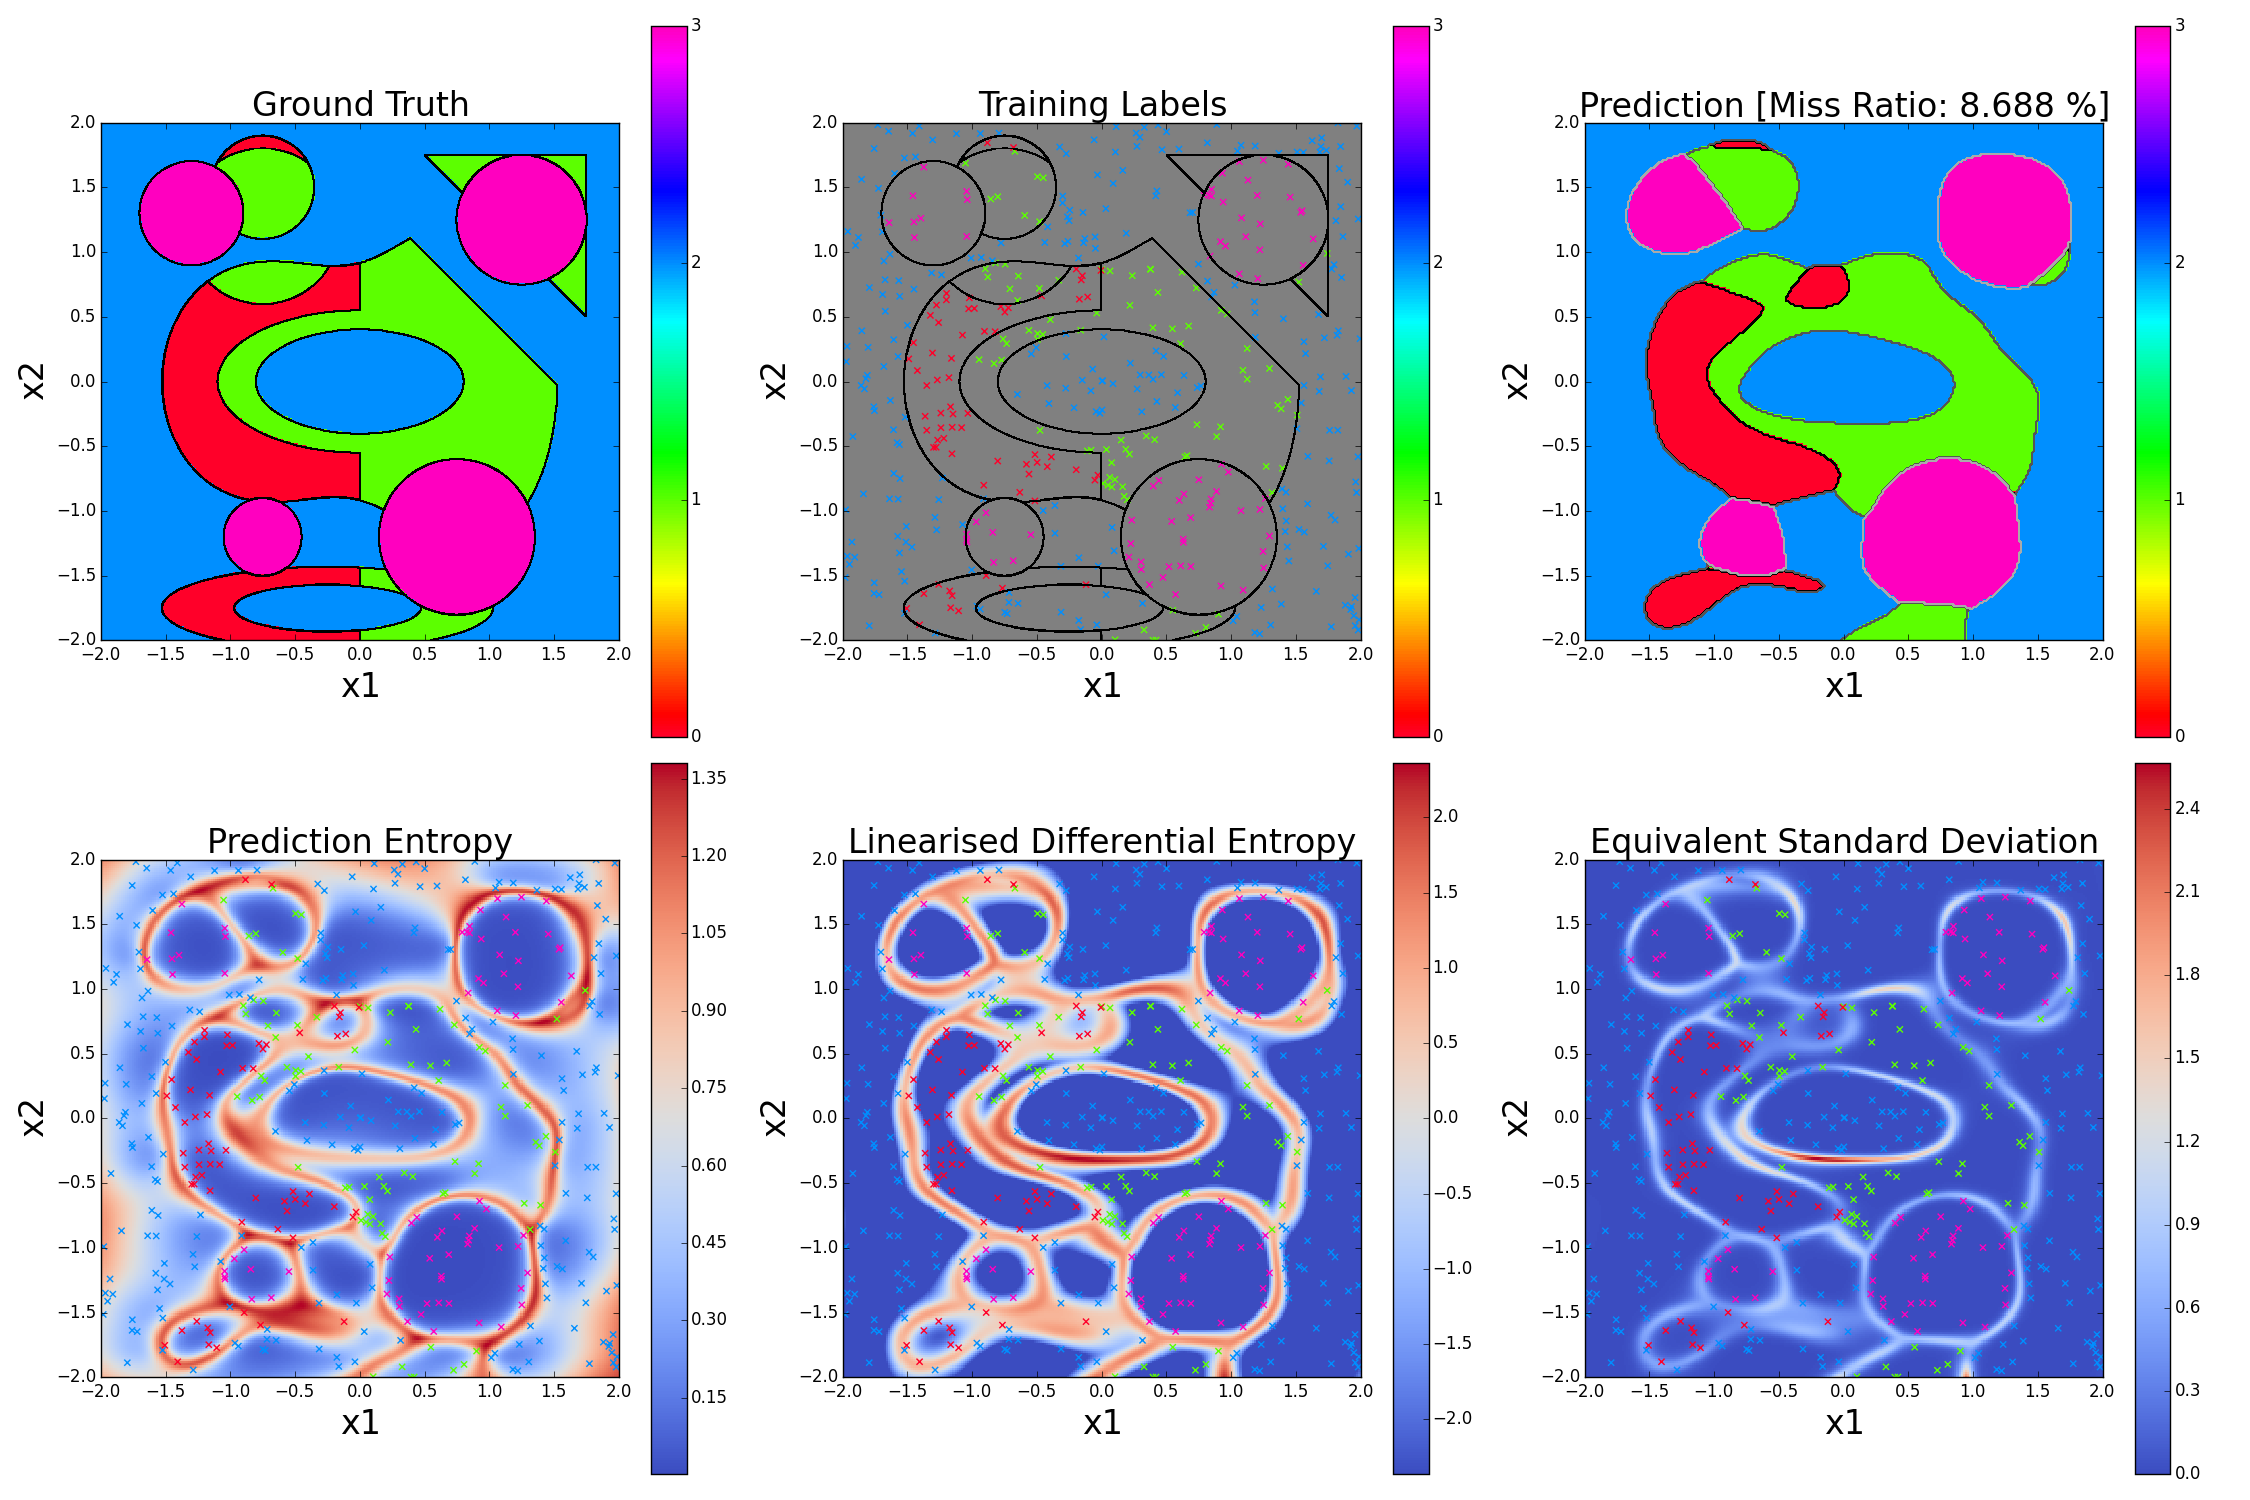
\includegraphics[width = \linewidth]{Figures/multiclass_linearised_entropy/Figure1.png}
		\caption{Example: Linearised Differential Entropy for a Multiclass Classifier}
		\label{Figure:Results:MulticlassLinearisedEntropy}
		\end{figure*}
			
		For multiclass classification, linearisation is performed on the softmax response functions which returns the predictive class probability $\vec{\pi}^{m}$ for each of the $c$ classes \eqref{Section:LinearisedEntropy:Equation:Softmax}. For notational clarity we move the query star ($^\star$) to the left and use the superscript $m$ to index the classes. The latent vector $\bvec{f}_{i}$ represents the collection of $c$ latent values across classes at the query point $i$, and is distinct from $\vec{f}_{m}$ which represents the collection of $n^{\star}$ latent values across query points for class $m$.

		\begin{equation}
			^{\star}\pi^{m}_{i} = \sigma(^{\star}\bvec{f}_{i}) := \frac{\exp(^{\star}f^{m}_{i})}{\sum_{k = 1}^{c} \exp(^{\star}f^{k}_{i})} \qquad m \in \{1, 2, \dots, c\}
		\label{Section:LinearisedEntropy:Equation:Softmax}
		\end{equation}	
					
		\subsubsection{Derivation}
		
		{\color{BurntOrange} This is a random paragraph of stuff. I talk about things. This is just a filler paragraph. Today is sunny. Rainbows are colorful. Blah blah blah.}
		
		{\color{BurntOrange} This is a random paragraph of stuff. I talk about things. This is just a filler paragraph. Today is sunny. Rainbows are colorful. Blah blah blah.}
		
		{\color{BurntOrange} This is a random paragraph of stuff. I talk about things. This is just a filler paragraph. Today is sunny. Rainbows are colorful. Blah blah blah.}
		
		{\color{BurntOrange} This is a random paragraph of stuff. I talk about things. This is just a filler paragraph. Today is sunny. Rainbows are colorful. Blah blah blah.}
		
		{\color{BurntOrange} This is a random paragraph of stuff. I talk about things. This is just a filler paragraph. Today is sunny. Rainbows are colorful. Blah blah blah.}
		
		{\color{BurntOrange} This is a random paragraph of stuff. I talk about things. This is just a filler paragraph. Today is sunny. Rainbows are colorful. Blah blah blah.}
		
		{\color{BurntOrange} This is a random paragraph of stuff. I talk about things. This is just a filler paragraph. Today is sunny. Rainbows are colorful. Blah blah blah.}
		
		{\color{BurntOrange} This is a random paragraph of stuff. I talk about things. This is just a filler paragraph. Today is sunny. Rainbows are colorful. Blah blah blah.}
		
		{\color{BurntOrange} This is a random paragraph of stuff. I talk about things. This is just a filler paragraph. Today is sunny. Rainbows are colorful. Blah blah blah.}
		
		{\color{BurntOrange} This is a random paragraph of stuff. I talk about things. This is just a filler paragraph. Today is sunny. Rainbows are colorful. Blah blah blah.}
		
		{\color{BurntOrange} This is a random paragraph of stuff. I talk about things. This is just a filler paragraph. Today is sunny. Rainbows are colorful. Blah blah blah.}
		
		{\color{BurntOrange} This is a random paragraph of stuff. I talk about things. This is just a filler paragraph. Today is sunny. Rainbows are colorful. Blah blah blah.}
		
		{\color{BurntOrange} This is a random paragraph of stuff. I talk about things. This is just a filler paragraph. Today is sunny. Rainbows are colorful. Blah blah blah.}
		
		{\color{BurntOrange} This is a random paragraph of stuff. I talk about things. This is just a filler paragraph. Today is sunny. Rainbows are colorful. Blah blah blah.}
		
		{\color{BurntOrange} This is a random paragraph of stuff. I talk about things. This is just a filler paragraph. Today is sunny. Rainbows are colorful. Blah blah blah.}
		
		{\color{BurntOrange} This is a random paragraph of stuff. I talk about things. This is just a filler paragraph. Today is sunny. Rainbows are colorful. Blah blah blah.}
		
	\subsection{Results}
		
		Here we compare the linearised differential entropy with the usual prediction information entropy of the Gaussian process classifier. For visualisation purposes, only the marginalised entropies are shown. We show examples where abundant information is available, where the difference in the properties in the two measures can be emphasized. 
		
		Figure \ref{Figure:Results:BinaryLinearisedEntropy} show a simple binary classification problem with abundant data, allowing a misclassification rate of only 3.298\%. The classifier is trained with a axis aligned Gaussian kernel with a probit response under Laplace approximation.
		
		Intuitively, under abundant data, we would like the classifier to only indicate high entropies at decision boundaries. In figure \ref{Figure:Results:BinaryLinearisedEntropy}, we see that the prediction information entropy is indeed near its maximum at the predict decision boundaries. However, it is also quite high around the edges where training data density is slightly lower, as there are no training points outside the region of interest that is shown. This suggests that if the prediction information entropy is used as the acquisition function for path planning, the vehicle would be suggested to spent some time travelling around the region of interest, collecting data it is already expecting. This is one of the fundamental properties of prediction information entropy - it is high at both predicted decision boundaries and also places with lower relative data density compared. 
		
		This leads to the classic exploration-exploitation dilemma most machine learning algorithms face. It is possible that there exists decision boundaries yet to be detected at regions of lower relative data density. Is it worth it for the vehicle to explore and discover such regions, or exploit the currently known boundaries and map it better? In most exploration applications, the priority is to map the region of interest as accurately and fast as possible in order to reduce time and cost. While it is possible that there exists undiscovered decision boundaries at regions of lower relative data density, it is undesirable under cost constraints that this possibility is weighed heavily by the vehicle even under abundant data.
		
		This demonstrates the advantage of linearised differential entropy. We can see in figure \ref{Figure:Results:BinaryLinearisedEntropy} that the linearised differential entropy is only high at the predicted decision boundaries. Note that the colour scale has been centred around zero differential entropy. Under such an acquisition function, the vehicle would focus strictly on the mapping the predicted decision boundaries better.
		
		Figure \ref{Figure:Results:MulticlassLinearisedEntropy} shows a similar scenario with a multi-class scenario with 4 labels. This classifier is trained through an one v.s. all approach with 4 binary classifiers using the same setup described above. Clearly the same behaviour as the binary case is observed, where the linearised differential entropy approach pushes down the entropy level of all regions except the predicted decision boundaries.
		

		

					
\section{Receding Horizon Approach to Informative Path Planning}
\label{Section:RecedingHorizonApproach}

	\subsection{Motivation}
	
	\subsection{Outline of Method}
	
	\subsection{Properties of the Receding Horizon Approach}
	
	\subsection{Results}
		\begin{figure}[!htbp]
		\centering
			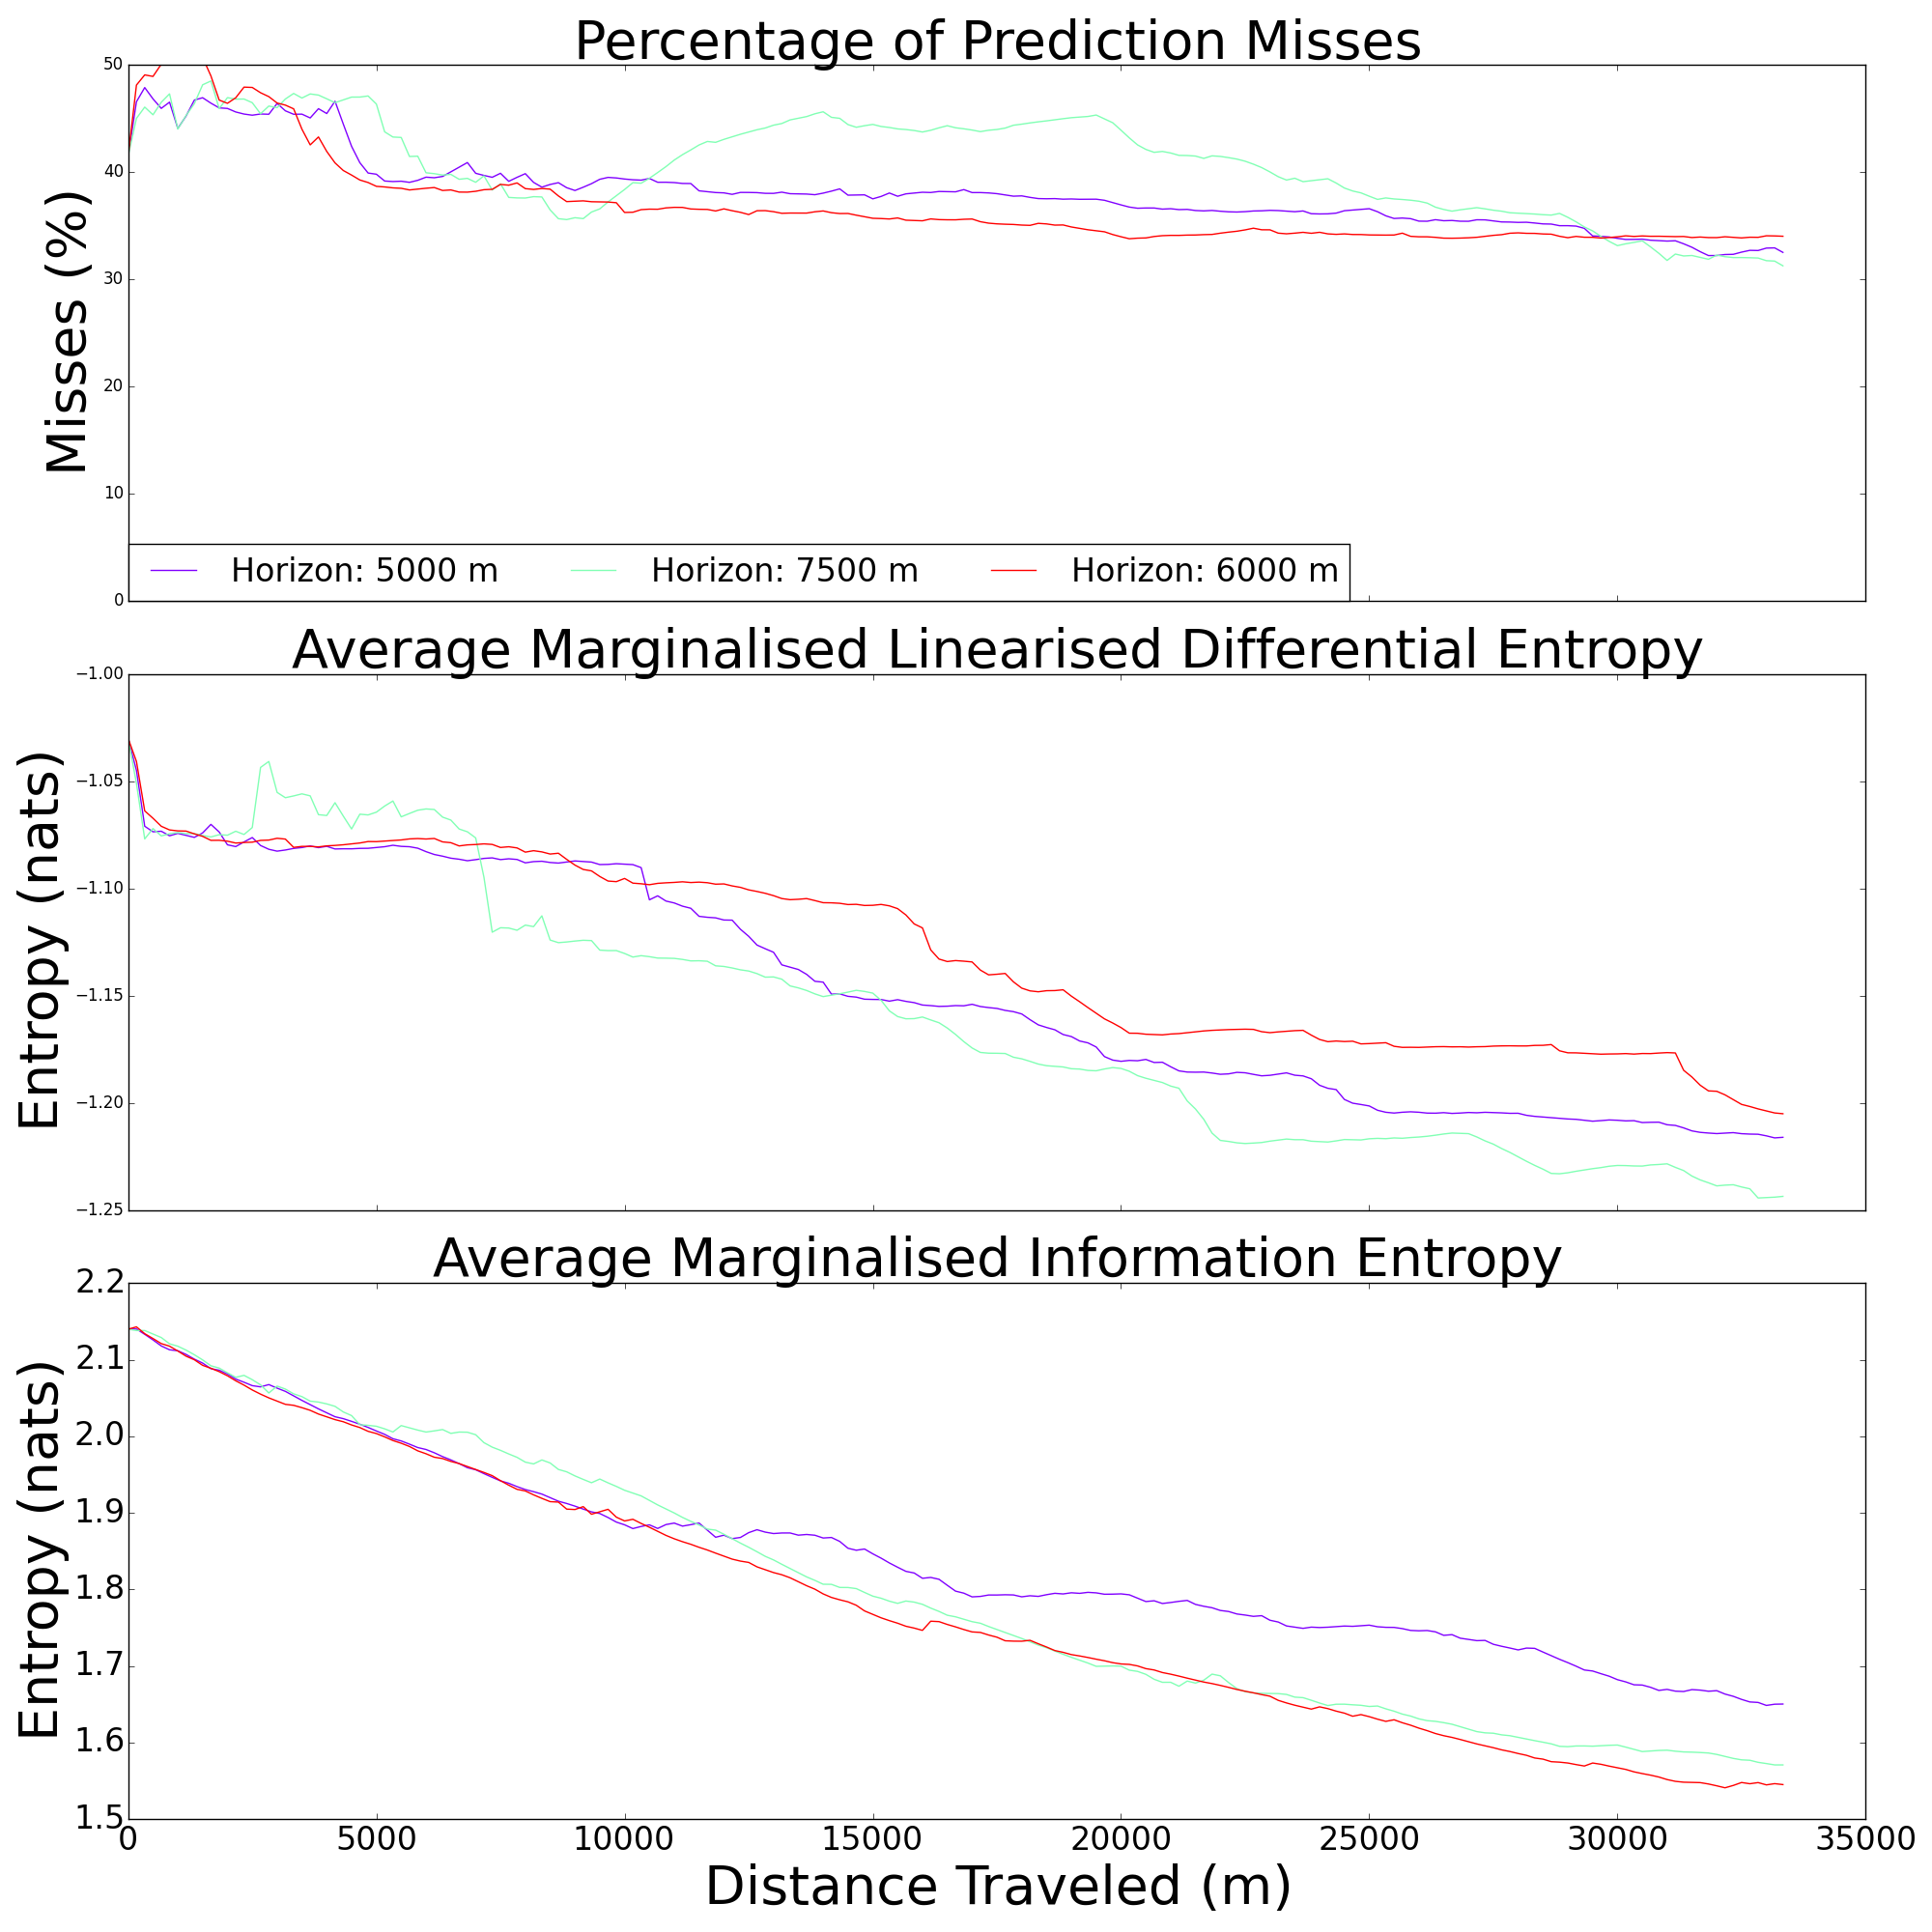
\includegraphics[width = \linewidth]{Figures/compare_horizons.png}
		\caption{Horizon Effects}
		\label{Figure:Results:CompareHorizons}
		\end{figure}
	
		\begin{figure}[!htbp]
		\centering
			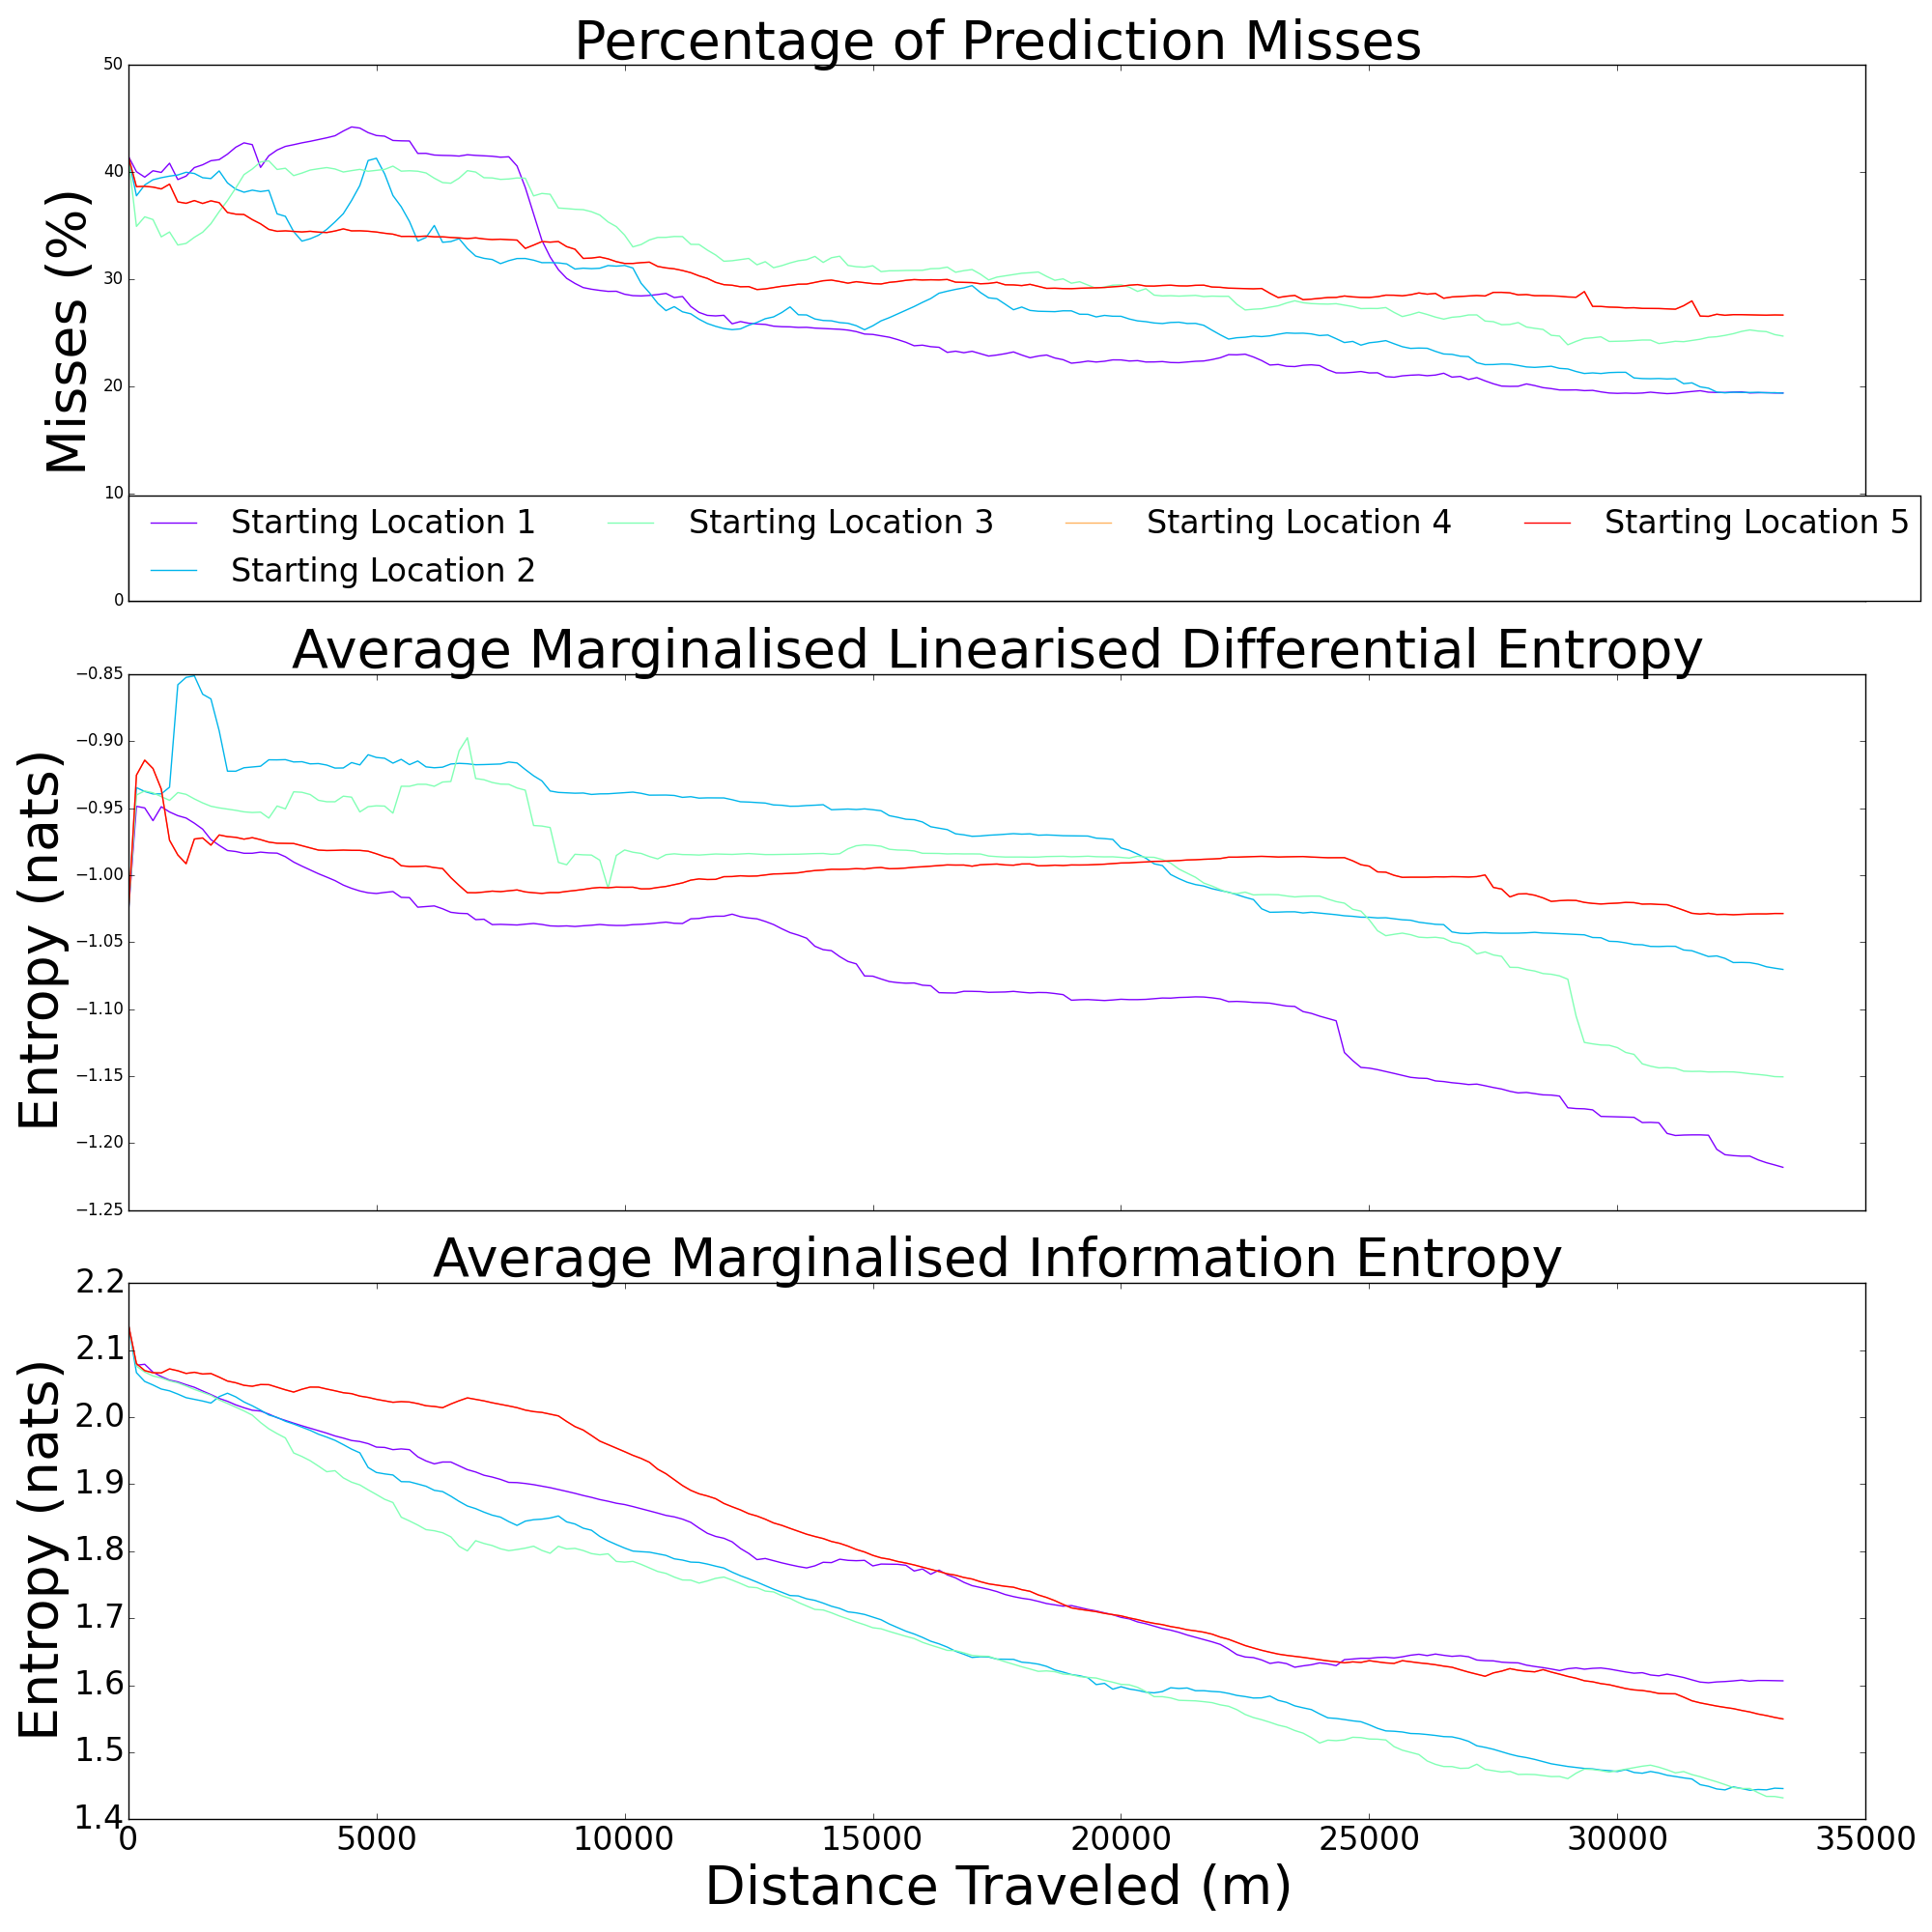
\includegraphics[width = \linewidth]{Figures/compare_locations.png}
		\caption{Horizon Effects}
		\label{Figure:Results:CompareLocations}
		\end{figure}
		
		\begin{figure}[!htbp]
		\centering
			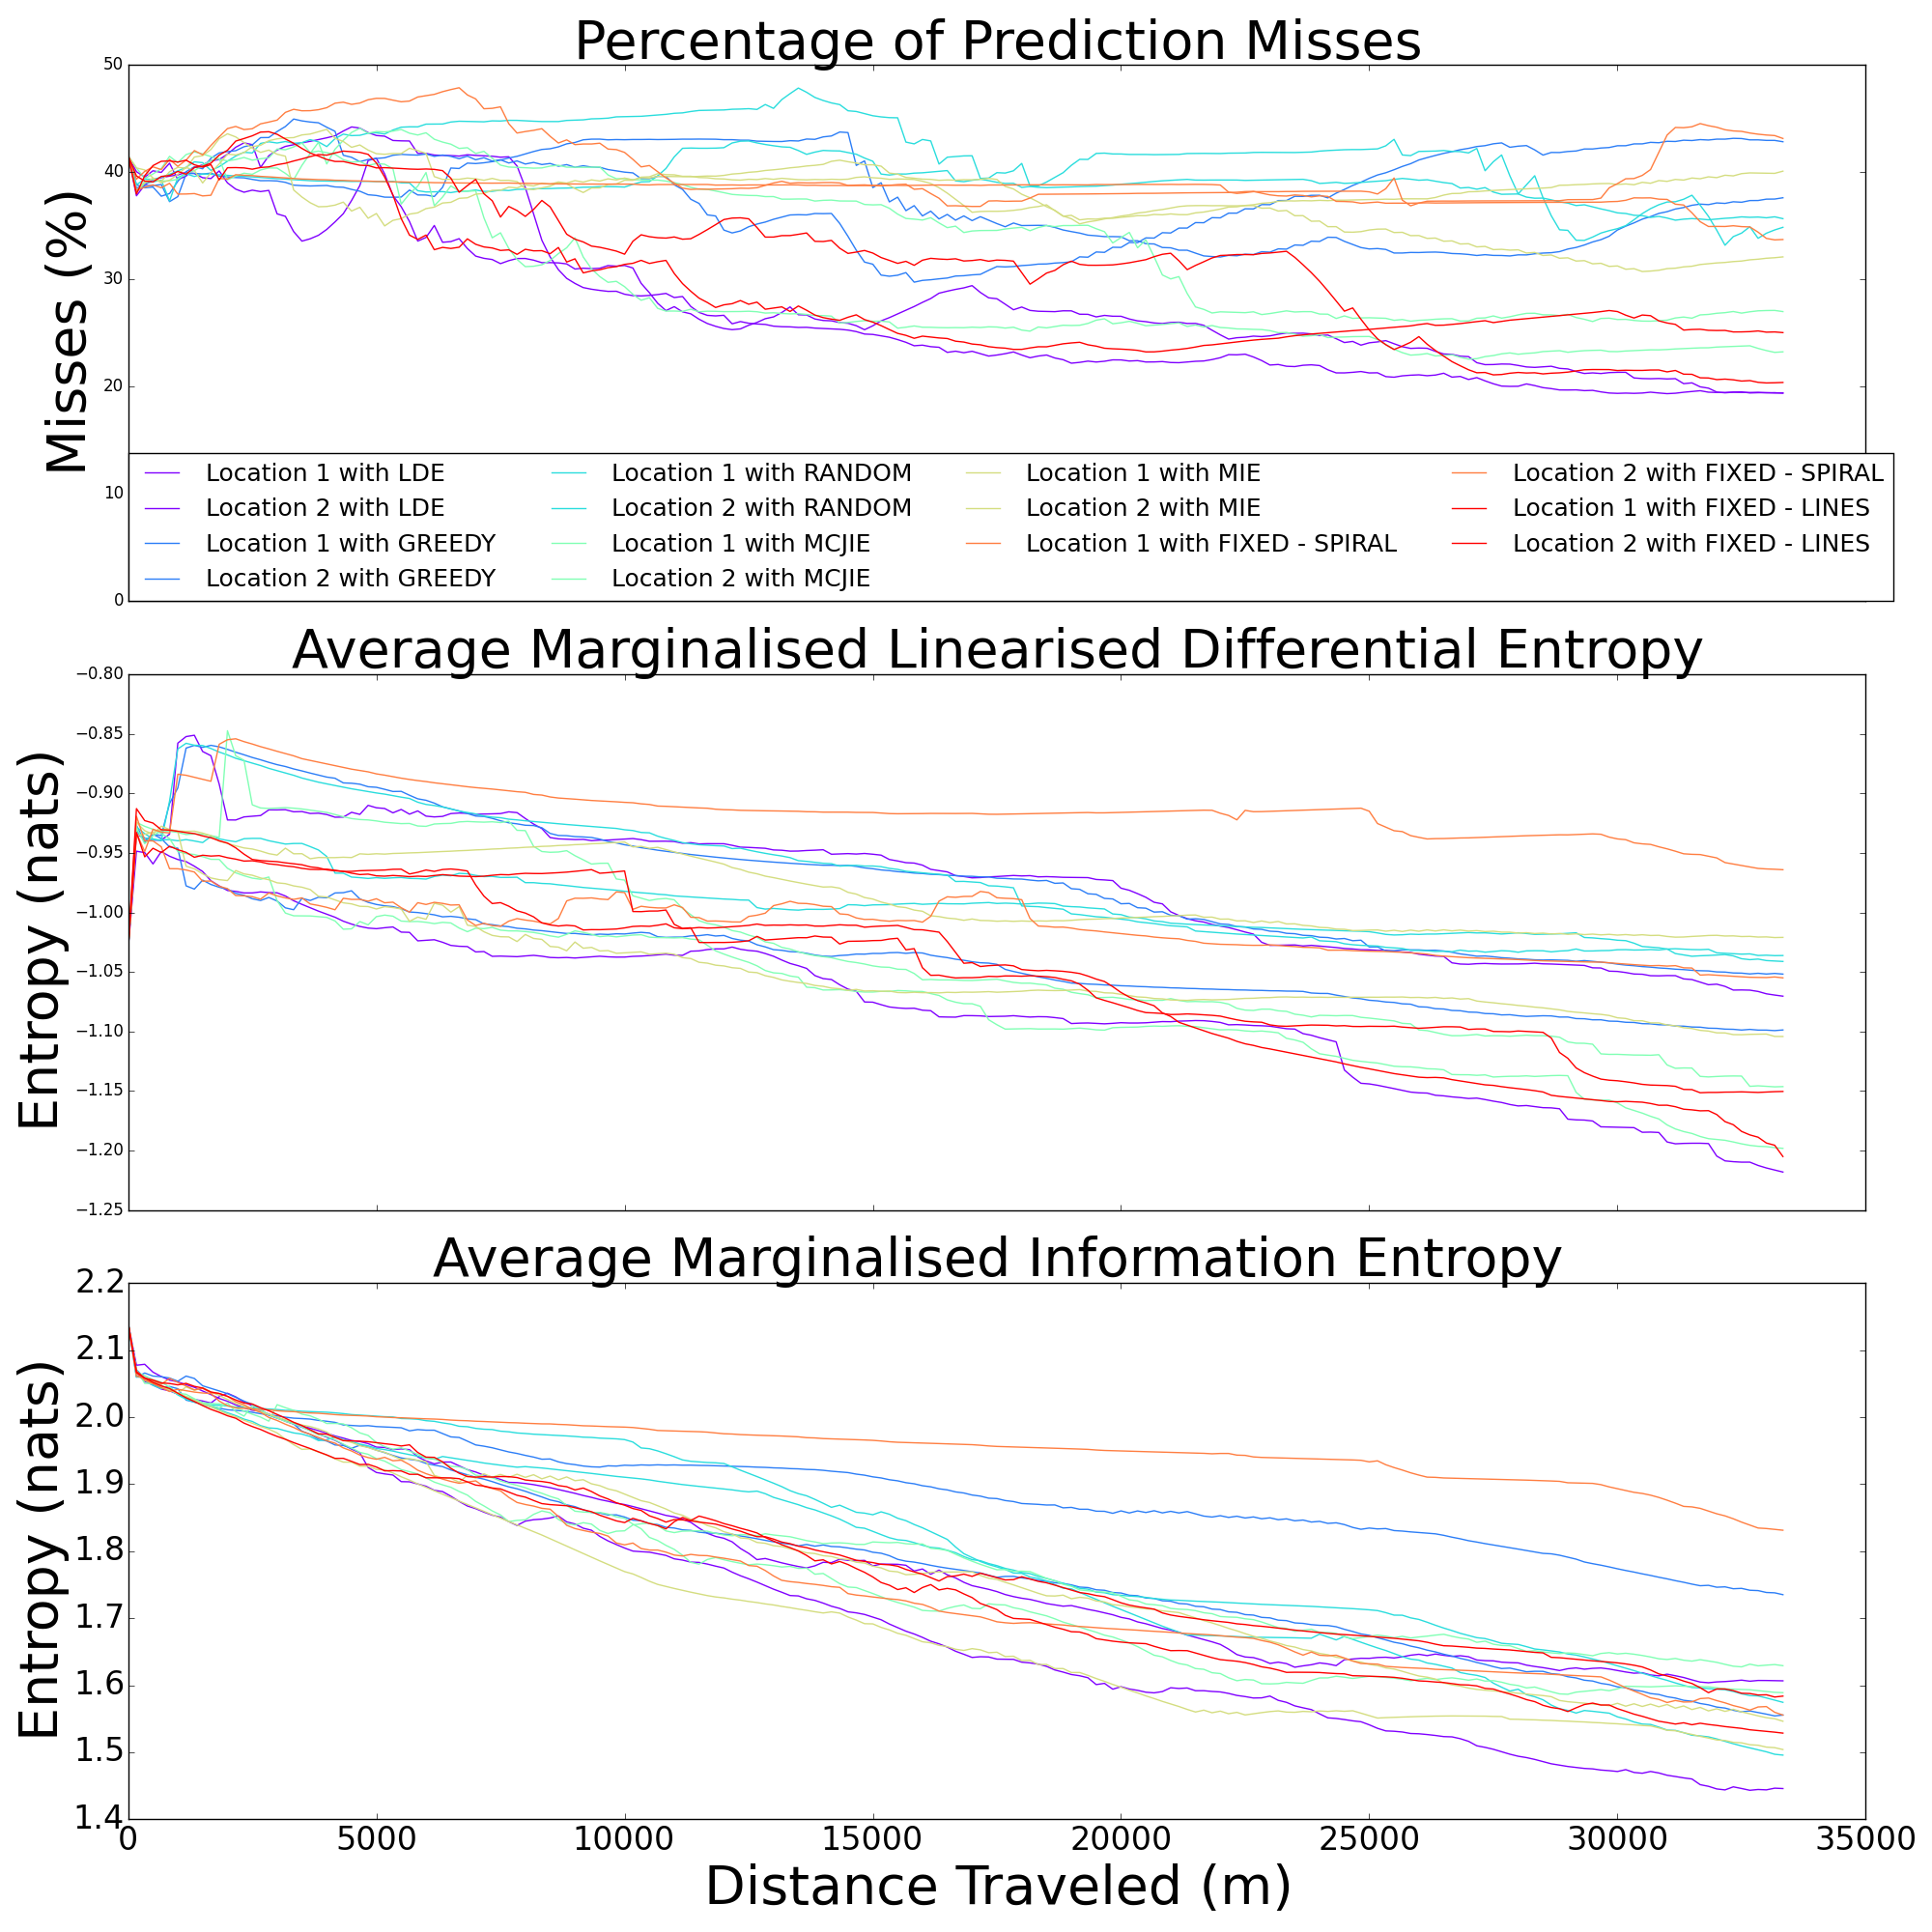
\includegraphics[width = \linewidth]{Figures/compare_methods.png}
		\caption{Horizon Effects}
		\label{Figure:Results:CompareMethods}
		\end{figure}
				
		From experimental tests:
			-A larger horizon is not always more beneficial. The entropy of faraway regions that it considers may become meaningless by the time it actually gets there, as the model would have significantly changed. On the other hand, it cannot be too short, or it will suffer the same problem as a greedy approach (not seeing ahead, getting stuck in local regions, not recognising joint information)
			-For the scott reef data, a good horizon range is 5000.0 m, for horizons more than 6000.0 m the result will hit diminishing returns and may actually hurt the performance. This happens as the model predictions and entropies at far away regions for which it was considering changes too much that during its way there the model has changed too much and it is no longer interested in such regions. This results in fast varying path proposals and may result in instability. It is about balancing obtaining reasonable information in reasonable time against reaching for information that may be outdated by the time it is collecting it.
			

		
		
\section{Conclusions and Future Work}
\label{Section:Conclusion}

\section*{Acknowledgments}


%% This section was initially prepared using BibTeX.  The .bbl file was
%% placed here later
%\bibliography{publications}
%\bibliographystyle{named}
%% The file named.bst is a bibliography style file for BibTeX 0.99c

\bibliographystyle{named}
\bibliography{acra2015}

\end{document}

